%\documentclass{beamer}
%\usepackage{amsmath}
%\usepackage{amsfonts}
%\usepackage{amsthm}
%\usepackage{amssymb}
%\usepackage{tikz}
%\usetikzlibrary{trees}
%\usepackage{lipsum}

%===== main document class =====
%\ifdefined\slideModeHandout
\documentclass%
[%
  handout,          % avoid unnecessary overlays
  aspectratio=169,  % aspect ratio fo 16:9 
  t,                % place content at top of frames
  10pt,             % use 10pt as standard font size (default size is 11pt)
  compress,         % compress things like navigation bars...
]{beamer}
%\else
%\documentclass%
%[%
%  aspectratio=169,  % aspect ratio fo 16:9 
%  t,                % place content at top of frames
%  10pt,             % use 10pt as standard font size (default size is 11pt)
%  compress,         % compress things like navigation bars...
%]{beamer}
%\fi

\mode<presentation>
%===============tabto==============
% tabto.sty
%
% version 1.4  (Dec 2018)
%
% Tabbing to fixed positions in a paragraph.
%
% Copyright 2006,2009,2012,2013,2018 by 
% Donald Arseneau,   Vancouver, Canada (asnd@triumf.ca)
% Permission to use, distribute and modify this software is granted
% under the conditions of the LaTeX Project Public License, either 
% version 1.3 or (at your option) any later version.  The license is
% found at http://www.latex-project.org/lppl.txt, and is part of all 
% recent distributions of LaTeX.
%
% This work has the LPPL maintenance status `maintained' (by author).
%
% Two new text positioning commands are defined: \tabto and \tab.
% 
% \tabto{<length>}
% Tab to a position relative to the left margin in a paragraph (any
% indentation due to a list or \leftskip is part of the `margin' in
% this context). If the text on the line already goes past the desired
% position, the tab starts a new line and moves to the requested
% horizontal position.
%
% \tabto*{<length>}
% Similar to \tabto, except it will perform backspacing, and over-
% print previous text on the line whenever that text is already
% longer than the specified length (i.e., no linebreak is produced).
% Line-breaks are suppressed immediately after \tabto or \tabto*.
%
% The length register "\CurrentLineWidth" will report the width
% of the existing text on the line, and it may be used in the
% <length> argument (using calc.sty, for example). Also, there
% is "\TabPrevPos" which gives the "\CurrentLineWidth" from the
% previous tab command (the position where the tab command occurred,
% not where it went to), and can be used to return to that position
% if no line breaks have occurred in between, or directly below it,
% if there were line breaks.
%
% \tab
% Tab to the next tab-stop chosen from a list of tab positions, in
% the traditional style of typewriters.  A \tab will always move
% to the next tab stop (or the next line), even if it is already
% exactly at a tab stop. Thus, "\tab" at the beginning of a line,
% or "\tab\tab" elsewhere skips a position. A linebreak is permitted 
% immediately following a \tab, in case the ensuing text does not 
% fit well in the remaining space.
%
% If you do not want to skip positions, use "\tabto{\NextTabStop}"
% instead of "\tab".  This is particularly useful when you want to
% use \tab in some other command, but do not want to skip a column
% for the first item.
%
% The tab-stop positions are declared using either \TabPositions
% or \NumTabs:
%
% \TabPositions{<length>, <length>,...<length>}
% Declares the tab stops as a comma-separated list of positions 
% relative to the left margin. A tab-stop at 0pt is implicit, and 
% need not be listed.
%
% \NumTabs{<number>}
% Declares a list of <number> equally-spaced tabs, starting at the
% left margin and spanning \linewidth.  For example \NumTabs{2} 
% declares tab-stops at 0pt and 0.5\linewidth, the same as
% \TabPositions{0pt, 0.5\linewidth} or \TabPositions{0.5\linewidth}
%
% After these declarations, the list of tab positions is saved in
% \TabStopList, and the next tab position, relative to the current 
% position, is given by \NextTabStop.  You do not normally need
% to access them, but they are available.
%
% Problems:
%
% Tall objects after a tab stop may overlap the line above, rather
% than forcing a greater separation between lines.

%\ProvidesPackage{tabto}[2018/12/28 \space v 1.4 \space 
%  Another tabbing mechanism]\relax

%%%%%%%%%Code Begin

%\newdimen\CurrentLineWidth
%\newdimen\TabPrevPos
%
%\newcommand\tabto[1]{%
% \leavevmode
% \begingroup
% \def\@tempa{*}\def\@tempb{#1}%
% \ifx\@tempa\@tempb % \tab* 
%   \endgroup
%   \TTo@overlaptrue % ... set a flag and re-issue \tabto to get argument
%   \expandafter\tabto
% \else
%   \ifinner % in a \hbox, so ignore
%   \else % unrestricted horizontal mode
%     \null% \predisplaysize will tell the position of this box (must be box)
%     \parfillskip\fill
%     \everydisplay{}\everymath{}%
%     \predisplaypenalty\@M \postdisplaypenalty\@M
%     $$% math display so we can test \predisplaysize
%      \lineskiplimit=-999pt % so we get pure \baselineskip
%      \abovedisplayskip=-\baselineskip \abovedisplayshortskip=-\baselineskip
%      \belowdisplayskip\z@skip \belowdisplayshortskip\z@skip
%      \halign{##\cr\noalign{%
%        % get the width of the line above
%        \ifdim\predisplaysize=\maxdimen %\message{Mixed R and L, so say the line is full. }%
%           \CurrentLineWidth\linewidth
%        \else
%           \ifdim\predisplaysize=-\maxdimen 
%             % \message{Not in a paragraph, so call the line empty. }%
%             \CurrentLineWidth\z@
%           \else
%             \ifnum\TTo@Direction<\z@
%               \CurrentLineWidth\linewidth \advance\CurrentLineWidth\predisplaysize
%             \else
%               \CurrentLineWidth\predisplaysize 
%             \fi
%             % Correct the 2em offset
%             \advance\CurrentLineWidth -2em
%             \advance\CurrentLineWidth -\displayindent
%             \advance\CurrentLineWidth -\leftskip
%        \fi\fi
%        \ifdim\CurrentLineWidth<\z@ \CurrentLineWidth\z@\fi
%        % Enshrine the tab-to position; #1 might reference \CurrentLineWidth
%        \setlength\@tempdimb{#1}% allow calc.sty
%        %\message{*** Tab to \the\@tempdimb, previous width is \the\CurrentLineWidth. ***}%
%        % Save width for possible return use
%        \global\TabPrevPos\CurrentLineWidth
%        % Build the action to perform
%        \protected@xdef\TTo@action{%
%           \vrule\@width\z@\@depth\the\prevdepth
%           \ifdim\CurrentLineWidth>\@tempdimb
%              \ifTTo@overlap\else
%                 \protect\newline \protect\null
%           \fi\fi
%           \protect\nobreak
%           \protect\hskip\the\@tempdimb\relax
%        }%
%        %\message{\string\TTo@action: \meaning \TTo@action. }%
%        % get back to the baseline, regardless of its depth.
%        \vskip-\prevdepth
%        \prevdepth-99\p@
%        \vskip\prevdepth
%      }}%
%      $$
%     % Don't count the display as lines in the paragraph
%     \count@\prevgraf \advance\count@-4 \prevgraf\count@
%     \TTo@action
%     %%   \penalty\@m % to allow a penalized line break
%   \fi
%   \endgroup
%   \TTo@overlapfalse
%   \ignorespaces
% \fi
%}
%
%% \tab -- to the next position
%% \hskip so \tab\tab moves two positions
%% Allow a (penalized but flexible) line-break right after the tab.
%%
%\newcommand\tab{\leavevmode\hskip2sp\tabto{\NextTabStop}%
%  \nobreak\hskip\z@\@plus 30\p@\penalty4000\hskip\z@\@plus-30\p@\relax}
%
%
%% Expandable macro to select the next tab position from the list
%
%\newcommand\NextTabStop{%
%  \expandafter \TTo@nexttabstop \TabStopList,\maxdimen,>%
%}
%
%\def\TTo@nexttabstop #1,{%
%    \ifdim#1<\CurrentLineWidth
%      \expandafter\TTo@nexttabstop
%    \else
%      \ifdim#1<0.9999\linewidth#1\else\z@\fi
%      \expandafter\strip@prefix
%    \fi
%}
%\def\TTo@foundtabstop#1>{}
%
%\newcommand\TabPositions[1]{\def\TabStopList{\z@,#1}}
%
%\newcommand\NumTabs[1]{%
%   \def\TabStopList{}%
%   \@tempdimb\linewidth 
%   \divide\@tempdimb by#1\relax
%   \advance\@tempdimb 1sp % counteract rounding-down by \divide
%   \CurrentLineWidth\z@
%   \@whiledim\CurrentLineWidth<\linewidth\do {%
%     \edef\TabStopList{\TabStopList\the\CurrentLineWidth,}%
%     \advance\CurrentLineWidth\@tempdimb
%   }%
%   \edef\TabStopList{\TabStopList\linewidth}%
%}
%
% %default setting of tab positions:
%\TabPositions{\parindent,.5\linewidth}
%
%%\newif\ifTTo@overlap \TTo@overlapfalse
%
%%\@ifundefined{predisplaydirection}{
%% \let\TTo@Direction\predisplaysize
%% \let\predisplaydirection\@undefined
%%}{
%% \let\TTo@Direction\predisplaydirection
%%}
%
%

% ===== include packages =====
\usepackage{lmodern}
\usepackage[utf8]{inputenc}      % Unicode UTF-8 encoding support
\usepackage[T2A,T1]{fontenc}         % T1 font encoding
\usepackage{etoolbox}            % Programming tools (used for \insertpartstartframe, \insertpartendframe)
\usepackage{ifthen}              % Simple conditional statements
\usepackage{amsmath}             % AMS math package
\usepackage{amssymb}             % Extended collection of math symbols
\usepackage{mathtools}           % More math stuff
\usepackage{nicefrac}            % Nice fractions
\usepackage{xcolor}              % Driver independent colors
\usepackage{colortbl}            % rowcolor for tables
\usepackage{array}               % tables and arrays with extended features (e.g., overlays)
\usepackage{makecell}            % Simple formatting of single table cells
\usepackage{multirow}            % Multi-rows in tabular environments
\usepackage{booktabs}            % More flexible lines for tabular environments
\usepackage{tabto}               % Easy way of specifying tabulators
\usepackage{adjustbox}           % Macros for adjusting boxed content (used in defining \fitbox)
\usepackage{relsize}             % Relative font sizes (\larger=\relsize{1}, \smaller=\relsize{-1})
\usepackage{graphicx}            % Inserting pictures
\usepackage{hyperref}            % Cross referencing
%\usepackage{media9}              % Include media objects
%\usepackage{animate}             % Animations
\usepackage{tikz}                % TikZ library for drawing
\usepackage{pgfplots}            % Plots
\usepackage{import}              % including stuff with relative paths
%\usepackage{listings}            % source code inclusion

%===== TikZ libraries =====
\usetikzlibrary{shapes}          % Additional shapes: Ellipse
\usetikzlibrary{shapes.symbols}  % Additional shapes: Symbols (e.g., "cloud")
\usetikzlibrary{shapes.arrows}   % Additional shapes: Arrows (e.g., "single arrow")
\usetikzlibrary{arrows}          % Arrow tips
\usetikzlibrary{arrows.meta}     % Adjustable arrow heads
\usetikzlibrary{positioning}     % Relative positioning of nodes

%===== pgfsetting =====
\pgfplotsset{compat=newest}      % Use newest version of pgf
\usepgfplotslibrary{fillbetween} % filling between curves

%===== nice tables =====
\setlength{\heavyrulewidth}{0.08em}
\setlength{\lightrulewidth}{0.08em}
\setlength{\cmidrulewidth}{0.04em}
\setlength{\aboverulesep}{0.4ex}
\setlength{\belowrulesep}{0.6ex}
\newcommand{\cmidbeg}{\addlinespace[0.40ex]}
\newcommand{\cmidend}{\addlinespace[0.10ex]}

\usepackage{caption}
\usepackage{subcaption}


%%%%%%%%%%%%%%%%%%%%%%%%%%%%%%%%%%%%%%%%%%%%%%%%%%%%%%%%%%%%
%%%%%%
%%%%%%     M A I N   D O C U M E N T   S W I T C H E S     
%%%%%%
%%%%%%%%%%%%%%%%%%%%%%%%%%%%%%%%%%%%%%%%%%%%%%%%%%%%%%%%%%%%

% define command for directly using switches
\newcommand{\usetoggle}[1]{\iftoggle{#1}{true}{false}}

% define switches
\newtoggle{useNavSymbols}               % display of navigation symbols
\newtoggle{useShadows}                  % use blocks with shadows
\newtoggle{useColorBlocks}              % use colored blocks
\newtoggle{useColorBlockTitles}         % use colored block titles
\newtoggle{useInverseBlockTitles}       % use colored block title background with white text
\newtoggle{altColors}                   % use alternative color theme
\newtoggle{addExercises}                % whether exercises are used
\newtoggle{specialHeiko}                % special stuff for Heiko
\newtoggle{specialThomas}               % special stuff for Thomas

\def\slideStyleThomas{..}


\ifdefined\slideStyleThomas

  %>>>>>>>>>> parameters for Thomas >>>>>>>>>>
  \title%
      [Image and Video Coding]%
      {Image and Video Coding I:\\[0.5ex] Fundamentals}
  \author%
      [T. Wiegand, J. Pfaff, J. Rasch]%
      {Thomas Wiegand, Jonathan Pfaff, Jennifer Rasch}
  \institute%
      [TU Berlin, Fraunhofer HHI]%
      {Technische Universität Berlin, Fraunhofer Heinrich Hertz Institute, Berlin}

  \newcommand{\slideOrganization}{}

  \settoggle{useNavSymbols}        {false}
  \settoggle{useShadows}           {true}
  \settoggle{useColorBlocks}       {true}
  \settoggle{useColorBlockTitles}  {true}
  \settoggle{useInverseBlockTitles}{true}
  \settoggle{altColors}            {false}
  \settoggle{addExercises}         {false}

  \settoggle{specialHeiko}         {false}
  \settoggle{specialThomas}        {true}
  %<<<<<<<<<< parameters for Thomas <<<<<<<<<<

\else

  %>>>>>>>>>> parameters for Heiko >>>>>>>>>>
  \title%
      {Data Compression}
  \author%
      [Heiko Schwarz]%
      {Heiko Schwarz}
  \institute%
      [Freie Universität Berlin]%
      {Freie Universität Berlin\\%
      Fachbereich Mathematik und Informatik}

\ifdefined\slideModeHandout
  \settoggle{useNavSymbols}        {false}
\else
  \settoggle{useNavSymbols}        {false}
\fi
  \settoggle{useShadows}           {true}
  \settoggle{useColorBlocks}       {true}
  \settoggle{useColorBlockTitles}  {true}
  \settoggle{useInverseBlockTitles}{true}
  \settoggle{altColors}            {false}
  \settoggle{addExercises}         {true}

  \settoggle{specialHeiko}         {true}
  \settoggle{specialThomas}        {false}
  %<<<<<<<<<< parameters for Heiko <<<<<<<<<<

\fi % end of conditional





%%%%%%%%%%%%%%%%%%%%%%%%%%%%%%%%%%%%%%%%%%%%%%%%%
%%%%%%
%%%%%%     C U S T O M I Z E   D E S I G N
%%%%%%
%%%%%%%%%%%%%%%%%%%%%%%%%%%%%%%%%%%%%%%%%%%%%%%%%

%===== spacing for lists and paragraphs (modified copy from beamerbaselocalstructure.sty) =====
\makeatletter
\setlength  \parskip         {2ex}
\setlength  \leftmargini     {2em}
\setlength  \leftmarginii    {2em}
\setlength  \leftmarginiii   {2em}
\setlength  \labelsep        {.5em}
\setlength  \labelwidth      {\leftmargini}
\addtolength\labelwidth      {-\labelsep}
\def\@listi  {\leftmargin\leftmargini
              \partopsep  \parskip
              \parskip    0.0\p@
              \parsep     0.0\p@
              \topsep     3.0\p@ \@plus1.0\p@ \@minus2.0\p@
              \itemsep    3.0\p@ \@plus1.0\p@ \@minus2.0\p@}
\let\@listI\@listi
\def\@listii {\leftmargin\leftmarginii
              \parsep     0.0\p@
              \topsep     3.0\p@ \@plus1.0\p@ \@minus2.0\p@
              \itemsep    3.0\p@ \@plus1.0\p@ \@minus2.0\p@}
\def\@listiii{\leftmargin\leftmarginiii
              \parsep     0.0\p@
              \topsep     3.0\p@ \@plus1.0\p@ \@minus2.0\p@
              \itemsep    3.0\p@ \@plus1.0\p@ \@minus2.0\p@}
\makeatother


%===== counter for exercises =====
\newcounter{exercise}


%===== enumerate symbols (modified copy from beamerbaseauxtemplates.sty) =====
\makeatletter

%--- define commands for changing enum style ---
\newcommand{\setenumstyledepth}[2]{% {enumdepth}{command for displaying counter}
  \ifthenelse{\equal{#1}{1}}%
     {\renewcommand*{\theenumi}{#2{enumi}}}%
     {\ifthenelse{\equal{#1}{2}}%
        {\renewcommand*{\theenumii}{#2{enumii}}}%
        {\renewcommand*{\theenumiii}{#2{enumiii}}}%
     }%
}
% Note: For the following command you can also use your own styles.
%       For example, a style "A." in a smaller font can be defined by
%         \newcommand{\AlphaDot}[1]{{\smaller\smaller\Alph{#1}.}}
\newcommand{\enumStyle}[1]{\setenumstyledepth{\the\@enumdepth}{#1}}
\newcommand{\enumStylesDefault}[3]{%
  \setenumstyledepth{1}{#1}%
  \setenumstyledepth{2}{#2}%
  \setenumstyledepth{3}{#3}%
}

%--- define commands for putting enum symbols ---
\newcommand{\putenumsquare}[1]{%
  \smaller%
  \usebeamercolor[bg]{\beameritemnestingprefix item projected}%
  \begin{pgfpicture}{-1ex}{-0.25ex}{1.1ex}{2.0ex}%
    \pgfpathrectangle{\pgfpoint{-1.2ex}{-0.6ex}}{\pgfpoint{2.4ex}{2.4ex}}%
    \pgfusepath{fill}%
    \pgftext[base,y=-0.15ex]{\color{fg}#1}%
  \end{pgfpicture}%
}
\newcommand{\putenumcircle}[1]{%
  \smaller%
  \usebeamercolor[bg]{\beameritemnestingprefix item projected}%
  \begin{pgfpicture}{-1ex}{-0.25ex}{1.1ex}{2.0ex}%
    \pgfpathcircle{\pgfpoint{0pt}{.6ex}}{1.3ex}%
    \pgfusepath{fill}%
    \pgftext[base,y=-0.15ex]{\color{fg}#1}%
  \end{pgfpicture}%
}
\newcommand{\putenumblank}[1]{%
  \smaller%
  \begin{pgfpicture}{-1ex}{-0.25ex}{1.1ex}{2.0ex}%
    \pgfpathrectangle{\pgfpoint{-1.2ex}{-0.6ex}}{\pgfpoint{2.4ex}{2.4ex}}%
    \pgftext[base,y=-0.15ex]{#1}%
  \end{pgfpicture}%
}
\newcommand{\putenumbracket}[1]{%
  \smaller%
  \begin{pgfpicture}{-1ex}{-0.25ex}{1.1ex}{2.0ex}%
    \pgfpathrectangle{\pgfpoint{-1.2ex}{-0.6ex}}{\pgfpoint{2.4ex}{2.4ex}}%
    \pgftext[base,y=-0.15ex]{$\boldsymbol{\langle}$#1$\boldsymbol{\rangle}$}%
  \end{pgfpicture}%
}
\newcommand{\putenumautoi}[1]{\putenumcircle{#1}}
\newcommand{\putenumautoii}[1]{\putenumcircle{#1}}
\newcommand{\putenumautoiii}[1]{\putenumcircle{#1}}
\newcommand{\putenumauto}[1]{%
  \ifthenelse{\equal{\the\@itemdepth}{1}}%
     {\putenumautoi{#1}}%
     {\ifthenelse{\equal{\the\@itemdepth}{2}}%
        {\putenumautoii{#1}}%
        {\putenumautoiii{#1}}%
     }%
}

%--- define beamer enum templates [square][circle][blank][bracket][auto] ---
\expandafter\let\csname beamer@@tmpop@enumerate item@square\endcsname\relax
\expandafter\let\csname beamer@@tmpop@enumerate subitem@square\endcsname\relax
\expandafter\let\csname beamer@@tmpop@enumerate subsubitem@square\endcsname\relax
\expandafter\let\csname beamer@@tmpop@enumerate mini template@square\endcsname\relax

\expandafter\let\csname beamer@@tmpop@enumerate item@circle\endcsname\relax
\expandafter\let\csname beamer@@tmpop@enumerate subitem@circle\endcsname\relax
\expandafter\let\csname beamer@@tmpop@enumerate subsubitem@circle\endcsname\relax
\expandafter\let\csname beamer@@tmpop@enumerate mini template@circle\endcsname\relax

\defbeamertemplate{enumerate item}{square}{\putenumsquare{\insertenumlabel}}
\defbeamertemplate{enumerate subitem}{square}{\putenumsquare{\insertsubenumlabel}}
\defbeamertemplate{enumerate subsubitem}{square}{\putenumsquare{\insertsubsubenumlabel}}
\defbeamertemplate{enumerate mini template}{square}{\putenumsquare{\insertenumlabel}}

\defbeamertemplate{enumerate item}{circle}{\putenumcircle{\insertenumlabel}}
\defbeamertemplate{enumerate subitem}{circle}{\putenumcircle{\insertsubenumlabel}}
\defbeamertemplate{enumerate subsubitem}{circle}{\putenumcircle{\insertsubsubenumlabel}}
\defbeamertemplate{enumerate mini template}{circle}{\putenumcircle{\insertenumlabel}}

\defbeamertemplate{enumerate item}{blank}{\putenumblank{\insertenumlabel}}
\defbeamertemplate{enumerate subitem}{blank}{\putenumblank{\insertsubenumlabel}}
\defbeamertemplate{enumerate subsubitem}{blank}{\putenumblank{\insertsubsubenumlabel}}
\defbeamertemplate{enumerate mini template}{blank}{\putenumblank{\insertenumlabel}}

\defbeamertemplate{enumerate item}{bracket}{\putenumbracket{\insertenumlabel}}
\defbeamertemplate{enumerate subitem}{bracket}{\putenumbracket{\insertsubenumlabel}}
\defbeamertemplate{enumerate subsubitem}{bracket}{\putenumbracket{\insertsubsubenumlabel}}
\defbeamertemplate{enumerate mini template}{bracket}{\putenumbracket{\insertenumlabel}}

\defbeamertemplate{enumerate item}{auto}{\putenumauto{\insertenumlabel}}
\defbeamertemplate{enumerate subitem}{auto}{\putenumauto{\insertsubenumlabel}}
\defbeamertemplate{enumerate subsubitem}{auto}{\putenumauto{\insertsubsubenumlabel}}
\defbeamertemplate{enumerate mini template}{auto}{\putenumauto{\insertenumlabel}}

%--- define commands for easily changing enum modes ---
% The outcommented simple version has a problem with enum nested in itemize (wrong level)
%   \newcommand{\enumMode}[1]{\setbeamertemplate{enumerate \beameritemnestingprefix item}[#1]} 
\newcommand{\enumMode}[1]{%
  \ifthenelse{\equal{\the\@enumdepth}{1}}%
     {\setbeamertemplate{enumerate item}[#1]}%
     {\ifthenelse{\equal{\the\@enumdepth}{2}}%
        {\setbeamertemplate{enumerate subitem}[#1]}%
        {\setbeamertemplate{enumerate subsubitem}[#1]}%
     }%
}
\newcommand{\enumAutoDefault}[3]{%
  \renewcommand*{\putenumautoi}[1]{\csname putenum#1\endcsname{##1}}%
  \renewcommand*{\putenumautoii}[1]{\csname putenum#2\endcsname{##1}}%
  \renewcommand*{\putenumautoiii}[1]{\csname putenum#3\endcsname{##1}}%
}

\makeatother



%===== itemize symbols (modified copy from beamerbaseauxtemplates.sty) =====
\makeatletter

%--- new item symbols ---
\newcommand{\isquare}{%
  \begin{pgfpicture}%
    \pgfpathrectangle{\pgfpointorigin}{\pgfpoint{1.0ex}{1.0ex}}%
    \pgfusepath{fill}%
    \pgfsetbaseline{-0.2ex}%
  \end{pgfpicture}%
}
\newcommand{\icircle}{%
  \begin{pgfpicture}%
    \pgfpathcircle{\pgfpoint{0pt}{.5ex}}{0.5ex}%
    \pgfusepath{fill}%
    \pgfsetbaseline{-0.2ex}%
  \end{pgfpicture}%
}
\newcommand{\itriangle}{%
  \begin{pgfpicture}%
    \pgfpathmoveto{\pgfpointorigin}
    \pgfpathlineto{\pgfpoint{0.0ex}{1.0ex}}%
    \pgfpathlineto{\pgfpoint{1.0ex}{0.5ex}}%
    \pgfusepath{fill}%
    \pgfsetbaseline{-0.2ex}%
  \end{pgfpicture}%
}
\newcommand{\idash}{%
  \begin{pgfpicture}%
    \pgfpathrectangle{\pgfpoint{0.0ex}{0.4ex}}{\pgfpoint{1.0ex}{0.2ex}}%
    \pgfusepath{fill}%
    \pgfsetbaseline{-0.2ex}%
  \end{pgfpicture}%
}
\newcommand{\iarrow}{%
  \begin{pgfpicture}%
    \pgfpathmoveto{\pgfpointorigin}
    \pgfpathlineto{\pgfpoint{-0.80ex}{ 0.75ex}}%    (-hl)( ht)  % tl =      total length
    \pgfpathlineto{\pgfpoint{-0.80ex}{ 0.25ex}}%    (-hl)( tt)  % tt = half total thickness
    \pgfpathlineto{\pgfpoint{-2.00ex}{ 0.25ex}}%    (-tl)( tt)  % hl =      head length
    \pgfpathlineto{\pgfpoint{-2.00ex}{-0.25ex}}%    (-tl)(-tt)  % ht = half head thickness
    \pgfpathlineto{\pgfpoint{-0.80ex}{-0.25ex}}%    (-hl)(-tt)
    \pgfpathlineto{\pgfpoint{-0.80ex}{-0.75ex}}%    (-hl)(-ht)
    \pgfusepath{fill}%
  \end{pgfpicture}%
}
\newcommand{\idarrow}{%
  \begin{pgfpicture}%
    \pgfpathmoveto{\pgfpointorigin}
    \pgfpathlineto{\pgfpoint{-0.80ex}{ 0.75ex}}%    (-hl)( ht)  % tl =      total length
    \pgfpathlineto{\pgfpoint{-0.80ex}{ 0.25ex}}%    (-hl)( tt)  % tt = half total thickness
    \pgfpathlineto{\pgfpoint{-2.00ex}{ 0.25ex}}%    (-tl)( tt)  % hl =      head length
    \pgfpathlineto{\pgfpoint{-2.00ex}{ 0.75ex}}%
    \pgfpathlineto{\pgfpoint{-2.80ex}{ 0.00ex}}%
    \pgfpathlineto{\pgfpoint{-2.00ex}{-0.75ex}}%
    \pgfpathlineto{\pgfpoint{-2.00ex}{-0.25ex}}%    (-tl)(-tt)  % ht = half head thickness
    \pgfpathlineto{\pgfpoint{-0.80ex}{-0.25ex}}%    (-hl)(-tt)
    \pgfpathlineto{\pgfpoint{-0.80ex}{-0.75ex}}%    (-hl)(-ht)
    \pgfusepath{fill}%
  \end{pgfpicture}%
}

%--- define beamer item templates [square][circle][triangle][dash][arrow] ---
\expandafter\let\csname beamer@@tmpop@itemize item@square\endcsname\relax
\expandafter\let\csname beamer@@tmpop@itemize subitem@square\endcsname\relax
\expandafter\let\csname beamer@@tmpop@itemize subsubitem@square\endcsname\relax

\expandafter\let\csname beamer@@tmpop@itemize item@circle\endcsname\relax
\expandafter\let\csname beamer@@tmpop@itemize subitem@circle\endcsname\relax
\expandafter\let\csname beamer@@tmpop@itemize subsubitem@circle\endcsname\relax

\expandafter\let\csname beamer@@tmpop@itemize item@triangle\endcsname\relax
\expandafter\let\csname beamer@@tmpop@itemize subitem@triangle\endcsname\relax
\expandafter\let\csname beamer@@tmpop@itemize subsubitem@triangle\endcsname\relax

\defbeamertemplate{itemize item}{square}{\isquare}
\defbeamertemplate{itemize subitem}{square}{\isquare}
\defbeamertemplate{itemize subsubitem}{square}{\isquare}

\defbeamertemplate{itemize item}{circle}{\icircle}
\defbeamertemplate{itemize subitem}{circle}{\icircle}
\defbeamertemplate{itemize subsubitem}{circle}{\icircle}

\defbeamertemplate{itemize item}{triangle}{\itriangle}
\defbeamertemplate{itemize subitem}{triangle}{\itriangle}
\defbeamertemplate{itemize subsubitem}{triangle}{\itriangle}

\defbeamertemplate{itemize item}{dash}{\idash}
\defbeamertemplate{itemize subitem}{dash}{\idash}
\defbeamertemplate{itemize subsubitem}{dash}{\idash}

\defbeamertemplate{itemize item}{arrow}{\iarrow}
\defbeamertemplate{itemize subitem}{arrow}{\iarrow}
\defbeamertemplate{itemize subsubitem}{arrow}{\iarrow}

%--- define command for easily changing item styles ---
\newcommand{\itemMode}[1]{\setbeamertemplate{itemize \beameritemnestingprefix item}[#1]}

\makeatother



%===== commands for text highlighting  =====
% helping command
\newcommand{\setfontrm} {\fontshape{\rmdefault}\selectfont}
\newcommand{\setfontit} {\fontshape{\itdefault}\selectfont}
\newcommand{\setfontrs} {\fontseries{\mddefault}\selectfont}
\newcommand{\setfontbs} {\fontseries{\bfdefault}\selectfont}
\newcommand{\setfontrrm}{\fontseries{\mddefault}\fontshape{\rmdefault}\selectfont}
\newcommand{\setfontrit}{\fontseries{\mddefault}\fontshape{\itdefault}\selectfont}
\newcommand{\setfontbrm}{\fontseries{\bfdefault}\fontshape{\rmdefault}\selectfont}
\newcommand{\setfontbit}{\fontseries{\bfdefault}\fontshape{\itdefault}\selectfont}
% normal text attributes:
  % setting series
  \newcommand<>{\regu}  [1]{{\only#2{\setfontrs}#1}}
  \newcommand<>{\bold}  [1]{{\only#2{\setfontbs}#1}}
  % setting shape
  \newcommand<>{\norm}  [1]{{\only#2{\setfontrm}#1}}
  \newcommand<>{\ital}  [1]{{\only#2{\setfontit}#1}}
  % setting series and shape
  \newcommand<>{\rnorm} [1]{{\only#2{\setfontrrm}#1}}
  \newcommand<>{\rital} [1]{{\only#2{\setfontrit}#1}}
  \newcommand<>{\bnorm} [1]{{\only#2{\setfontbrm}#1}}
  \newcommand<>{\bital} [1]{{\only#2{\setfontbit}#1}}
% special text highlighting:
  % changing color only
\renewcommand<>{\alert} [1]{{\only#2{\usebeamercolor{alerted text}\color{fg}}#1}}
  \newcommand<>{\struc} [1]{{\only#2{\usebeamercolor{structure}\color{fg}}#1}}
  \newcommand<>{\examp} [1]{{\only#2{\usebeamercolor{example text}\color{fg}}#1}}
  % changing color and series
  \newcommand<>{\Alert} [1]{{\only#2{\setfontrs\usebeamercolor{alerted text}\color{fg}}#1}}
  \newcommand<>{\Struc} [1]{{\only#2{\setfontrs\usebeamercolor{structure}\color{fg}}#1}}
  \newcommand<>{\Examp} [1]{{\only#2{\setfontrs\usebeamercolor{example text}\color{fg}}#1}}
  \newcommand<>{\ALERT} [1]{{\only#2{\setfontbs\usebeamercolor{alerted text}\color{fg}}#1}}
  \newcommand<>{\STRUC} [1]{{\only#2{\setfontbs\usebeamercolor{structure}\color{fg}}#1}}
  \newcommand<>{\EXAMP} [1]{{\only#2{\setfontbs\usebeamercolor{example text}\color{fg}}#1}}
  % changing color and shape
  \newcommand<>{\ralert}[1]{{\only#2{\setfontrm\usebeamercolor{alerted text}\color{fg}}#1}}
  \newcommand<>{\rstruc}[1]{{\only#2{\setfontrm\usebeamercolor{structure}\color{fg}}#1}}
  \newcommand<>{\rexamp}[1]{{\only#2{\setfontrm\usebeamercolor{example text}\color{fg}}#1}}
  \newcommand<>{\ialert}[1]{{\only#2{\setfontit\usebeamercolor{alerted text}\color{fg}}#1}}
  \newcommand<>{\istruc}[1]{{\only#2{\setfontit\usebeamercolor{structure}\color{fg}}#1}}
  \newcommand<>{\iexamp}[1]{{\only#2{\setfontit\usebeamercolor{example text}\color{fg}}#1}}
  % changing color, shape, and series
  \newcommand<>{\rAlert}[1]{{\only#2{\setfontrrm\usebeamercolor{alerted text}\color{fg}}#1}}
  \newcommand<>{\rStruc}[1]{{\only#2{\setfontrrm\usebeamercolor{structure}\color{fg}}#1}}
  \newcommand<>{\rExamp}[1]{{\only#2{\setfontrrm\usebeamercolor{example text}\color{fg}}#1}}
  \newcommand<>{\rALERT}[1]{{\only#2{\setfontbrm\usebeamercolor{alerted text}\color{fg}}#1}}
  \newcommand<>{\rSTRUC}[1]{{\only#2{\setfontbrm\usebeamercolor{structure}\color{fg}}#1}}
  \newcommand<>{\rEXAMP}[1]{{\only#2{\setfontbrm\usebeamercolor{example text}\color{fg}}#1}}
  \newcommand<>{\iAlert}[1]{{\only#2{\setfontrit\usebeamercolor{alerted text}\color{fg}}#1}}
  \newcommand<>{\iStruc}[1]{{\only#2{\setfontrit\usebeamercolor{structure}\color{fg}}#1}}
  \newcommand<>{\iExamp}[1]{{\only#2{\setfontrit\usebeamercolor{example text}\color{fg}}#1}}
  \newcommand<>{\iALERT}[1]{{\only#2{\setfontbit\usebeamercolor{alerted text}\color{fg}}#1}}
  \newcommand<>{\iSTRUC}[1]{{\only#2{\setfontbit\usebeamercolor{structure}\color{fg}}#1}}
  \newcommand<>{\iEXAMP}[1]{{\only#2{\setfontbit\usebeamercolor{example text}\color{fg}}#1}}
% specials: Emphasizing and names [May want to redefine in actually used style]
\renewcommand<>{\emph}  [1]{\alert#2{#1}}
  \newcommand<>{\Emph}  [1]{\ALERT#2{#1}}
  \newcommand<>{\EMPH}  [1]{\iALERT#2{#1}}
  \newcommand  {\aname} [1]{{\rmfamily\scshape #1}}



%===== define subblock environments =====
\makeatletter
\newenvironment{nesting}{%
  \par\hspace{2\beamer@leftmargin}
  \begin{minipage}{\linewidth-\beamer@leftmargin-3.5\beamer@rightmargin}%
}{%
  \end{minipage}
}
\makeatother



%===== define hooks for accessing frame number inside part  =====
\makeatletter
\newcount\beamer@partstartframe
\beamer@partstartframe=1
\apptocmd{\beamer@part}{\addtocontents{nav}{\protect\headcommand{%
    \protect\beamer@partframes{\the\beamer@partstartframe}{\the\c@framenumber}}}}{}{}
\apptocmd{\beamer@part}{\beamer@partstartframe=\c@framenumber\advance\beamer@partstartframe by1\relax}{}{}
\AtEndDocument{\immediate\write\@auxout{\string\@writefile{nav}%
    {\noexpand\headcommand{\noexpand\beamer@partframes{\the\beamer@partstartframe}{\the\c@framenumber}}}}}{}{}
\def\beamer@startframeofpart{1}
\def\beamer@endframeofpart{1}
\def\beamer@partframes#1#2{%
    \ifnum\c@framenumber<#1%
    \else%
    \ifnum\c@framenumber>#2%
    \else%
    \gdef\beamer@startframeofpart{#1}%
    \gdef\beamer@endframeofpart{#2}%
    \fi%
    \fi%
}
\newcommand\insertpartstartframe{\beamer@startframeofpart}
\newcommand\insertpartendframe{\beamer@endframeofpart}
\makeatother
\def\inserttotalpartframenumber{%
    \pgfmathparse{(\insertpartendframe-\insertpartstartframe+1)}%
    \pgfmathprintnumber[fixed,precision=2]{\pgfmathresult}%
}
\def\insertpartframenumber{%
    \pgfmathparse{(\insertframenumber-\insertpartstartframe+1)}%
    \pgfmathprintnumber[fixed,precision=2]{\pgfmathresult}%
}



%===== define visible on macro for tikz pictures  =====
% see https://tex.stackexchange.com/questions/55806/mindmap-tikzpicture-in-beamer-reveal-step-by-step#55849
\tikzset{
  invisible/.style={opacity=0},
  visible on/.style={alt={#1{}{invisible}}},
  alt/.code args={<#1>#2#3}{%
    \alt<#1>{\pgfkeysalso{#2}}{\pgfkeysalso{#3}} % \pgfkeysalso doesn't change the path
  },
  action/.code args={<#1>#2}{%
    \action<#1>{\pgfkeysalso{#2}} % \pgfkeysalso doesn't change the path
  },
}
% see https://tex.stackexchange.com/questions/6135/how-to-make-beamer-overlays-with-tikz-node
\tikzset{onslide/.code args={<#1>#2}{% \pgfkeysalso doesn't change the path
  \only<#1>{\pgfkeysalso{#2}} %
}}
\tikzset{temporal/.code args={<#1>#2#3#4}{% \pgfkeysalso doesn't change the path
  \temporal<#1>{\pgfkeysalso{#2}}{\pgfkeysalso{#3}}{\pgfkeysalso{#4}} %
}}


%===== further helpful tikz macros =====
\newcommand{\budash}{{\tikz[baseline=0.1ex]\draw[thick](0,0)--({0.6em},0);}}
\newcommand{\nudash}{{\tikz[baseline=0.1ex]\draw[]     (0,0)--({0.6em},0);}}



%===== define a fitbox command  =====
\makeatletter
\newlength{\fitboxw}
\newlength{\fitboxh}
\newlength{\slideinnerheight}
\setlength{\slideinnerheight}{0.85\textheight} %%% could be reset later
\newcommand<>{\fitbox}[4][c]{%
  \only#5{%
    {%
      \setlength{\fitboxw}{#2}%
      \setlength{\fitboxh}{#3}%
      \parbox[#1][\fitboxh]{\fitboxw}{%
        \centering%
        \vfill%
        \adjustbox{%
          min width=\fitboxw,%
          min height=\fitboxh,%
          max width=\fitboxw,%
          max height=\fitboxh%
        }%
        {#4}%
        \vfill%
      }%
    }%
  }%
}
\newcommand<>{\hfitbox}[3][c]{%
  \only#4{%
    {%
      \setlength{\fitboxw}{#2}%
      \parbox[#1]{\fitboxw}{%
        \adjustbox{%
          min width=\fitboxw,%
          max width=\fitboxw}%
        {#3}%
      }%
    }%
  }%
}
\newcommand<>{\slidehfitbox}[1]{%
  \hfitbox#2{\textwidth}{#1}%
}
\newcommand<>{\slidefitbox}[1]{%
  \fitbox#2{\textwidth}{\slideinnerheight}{#1}%
}
\makeatother



%===== command for adding new part with part page / adding title page  =====
\newcommand{\startnewpart}[2][\usebeamercolor{background}\color{bg}\rule{1pt}{1pt}]{
  \part{#2}
  {
    \setbeamertemplate{navigation symbols}{}
    \begin{frame}[plain]
    \vfill\vfill
    {\hfill\begin{beamercolorbox}[%
       sep=8pt,dp=1ex,center,wd=0.8\textwidth,%
       rounded=true,
       shadow=\usetoggle{useShadows}%
    ]%
    {part title}
    \usebeamerfont{part title}\insertpart\par
    \end{beamercolorbox}\hfill}
    \vfill
    {\hfill{\fitbox{0.8\textwidth}{0.45\textheight}{#1}}\hfill}
    \vspace{0pt}
    \end{frame}
  }
}
\newcommand{\addtitlepage}{
  {
    \setbeamertemplate{navigation symbols}{}
    \begin{frame}[plain]
    \vspace{0.15\textheight}
    {\hfill\begin{beamercolorbox}[%
       sep=8pt,dp=1ex,center,wd=0.8\textwidth,%
       rounded=true,
       shadow=\usetoggle{useShadows}%
    ]%
    {title}
    \usebeamerfont{title}\inserttitle\par
    \end{beamercolorbox}\hfill}

    \begin{center}\large
      ~\\[3ex]
      {\insertauthor}\\[3ex]
      {\insertinstitute}
    \end{center}
    \end{frame}
  }
}







%%%%%%%%%%%%%%%%%%%%%%%%%%%%%%%%%%%%%%%%%%%
%%%%%%
%%%%%%     T E M P L A T E
%%%%%%
%%%%%%%%%%%%%%%%%%%%%%%%%%%%%%%%%%%%%%%%%%%

%===== other font size =====
\makeatletter
\newcommand\notsotiny{\@setfontsize\notsotiny\@vipt\@viipt}
\makeatother

%===== font theme =====
\usefonttheme{structurebold}
\setbeamerfont{title in head/foot}{size=\tiny}
\setbeamerfont{author in head/foot}{size=\tiny}
\setbeamerfont{date in head/foot}{size=\tiny}
\setbeamerfont*{frametitle}{family=\sffamily,series=\bfseries,shape=\upshape,size=\large}


%===== color theme (based on color theme "beaver") =====
%>>> define colors (see http://latexcolor.com/ for a good visual comparison)
% reds
\definecolor{bostonuniversityred}     {rgb}{0.80, 0.00, 0.00} % used in beaver
\definecolor{cornellred}              {rgb}{0.70, 0.11, 0.11}
\definecolor{red(ncs)}                {rgb}{0.77, 0.01, 0.20}
\definecolor{carmine}                 {rgb}{0.59, 0.00, 0.09}
\definecolor{crimsonglory}            {rgb}{0.75, 0.00, 0.20}
\definecolor{deepcarmine}             {rgb}{0.66, 0.13, 0.24}
\definecolor{harvardcrimson}          {rgb}{0.79, 0.00, 0.09}
\definecolor{lava}                    {rgb}{0.81, 0.06, 0.13}
\definecolor{mordantred19}            {rgb}{0.68, 0.05, 0.00}
\definecolor{persianred}              {rgb}{0.80, 0.20, 0.20}
\definecolor{raspberry}               {rgb}{0.89, 0.04, 0.36}
% greens                              
\definecolor{othergreen}              {rgb}{0.00, 0.80, 0.00}
\definecolor{officegreen}             {rgb}{0.00, 0.50, 0.00}
\definecolor{darkgreen}               {rgb}{0.00, 0.20, 0.13}
\definecolor{pakistangreen}           {rgb}{0.00, 0.40, 0.00}
\definecolor{cadmiumgreen}            {rgb}{0.00, 0.42, 0.24}
\definecolor{lincolngreen}            {rgb}{0.11, 0.35, 0.02}
\definecolor{dartmouthgreen}          {rgb}{0.05, 0.50, 0.06}
\definecolor{sacramentostategreen}    {rgb}{0.00, 0.34, 0.25}
\definecolor{tropicalrainforest}      {rgb}{0.00, 0.46, 0.37}
\definecolor{upforestgreen}           {rgb}{0.00, 0.27, 0.13}
\definecolor{lasallegreen}            {rgb}{0.03, 0.47, 0.19}
\definecolor{indiagreen}              {rgb}{0.07, 0.53, 0.03}
\definecolor{forestgreen(traditional)}{rgb}{0.00, 0.27, 0.13}
% blues                               
\definecolor{mediumblue}              {rgb}{0.00, 0.00, 0.80}
\definecolor{navyblue}                {rgb}{0.00, 0.00, 0.50}
\definecolor{ceruleanblue}            {rgb}{0.16, 0.32, 0.75}
\definecolor{internationalkleinblue}  {rgb}{0.00, 0.18, 0.65}
\definecolor{royalazure}              {rgb}{0.00, 0.22, 0.66}
\definecolor{smalt(darkpowderblue)}   {rgb}{0.00, 0.20, 0.60}
\definecolor{ultramarine}             {rgb}{0.07, 0.04, 0.56}
\definecolor{zaffre}                  {rgb}{0.00, 0.08, 0.66}
\definecolor{phthaloblue}             {rgb}{0.00, 0.06, 0.54}
\definecolor{persianblue}             {rgb}{0.11, 0.22, 0.73}
\definecolor{palatinateblue}          {rgb}{0.15, 0.23, 0.89}
% other
\definecolor{vividviolet}             {rgb}{0.62, 0.00, 1.00}
\definecolor{uclagold}                {rgb}{1.00, 0.70, 0.00}
\definecolor{tangerineyellow}         {rgb}{1.00, 0.80, 0.00}
\definecolor{shockingpink}            {rgb}{0.99, 0.06, 0.75}
\definecolor{schoolbusyellow}         {rgb}{1.00, 0.85, 0.00}
\definecolor{saddlebrown}             {rgb}{0.55, 0.27, 0.07}
\definecolor{purple(munsell)}         {rgb}{0.62, 0.00, 0.77}
\definecolor{portlandorange}          {rgb}{1.00, 0.35, 0.21}
\definecolor{persianrose}             {rgb}{1.00, 0.16, 0.64}
\definecolor{orange(colorwheel)}      {rgb}{1.00, 0.50, 0.00}
\definecolor{lightcyan}               {rgb}{0.88, 1.00, 1.00}
\definecolor{goldenyellow}            {rgb}{1.00, 0.87, 0.00}
\definecolor{electricindigo}          {rgb}{0.44, 0.00, 1.00}
\definecolor{darkorange}              {rgb}{1.00, 0.55, 0.00}
\definecolor{cyan(process)}           {rgb}{0.00, 0.72, 0.92}
\definecolor{aqua}                    {rgb}{0.00, 1.00, 1.00}
\definecolor{aquamarine}              {rgb}{0.50, 1.00, 0.83}
\definecolor{amber}                   {rgb}{1.00, 0.75, 0.00}
\definecolor{aliceblue}               {rgb}{0.94, 0.97, 1.00}


%===== specify main colors =====
\iftoggle{altColors}{%
  \colorlet{fgColorTheme}{bostonuniversityred}
  \colorlet{bgColorTheme}{gray}
  \colorlet{fgColorStruc}{royalazure}
  \colorlet{bgColorStruc}{bgColorTheme}
  \colorlet{fgColorAlert}{bostonuniversityred}
  \colorlet{bgColorAlert}{fgColorAlert}
  \colorlet{fgColorExamp}{indiagreen}
  \colorlet{bgColorExamp}{fgColorExamp}
}{%
  \colorlet{fgColorTheme}{royalazure}
  \colorlet{bgColorTheme}{gray}
  \colorlet{fgColorStruc}{royalazure}
  \colorlet{bgColorStruc}{bgColorTheme}
  \colorlet{fgColorAlert}{bostonuniversityred}
  \colorlet{bgColorAlert}{fgColorAlert}
  \colorlet{fgColorExamp}{indiagreen}
  \colorlet{bgColorExamp}{fgColorExamp}
}

% derived colors
\colorlet{fgColorThemedark}    {fgColorTheme!80!black}
\colorlet{fgColorThemeDark}    {fgColorTheme!70!black}
\colorlet{fgColorThemeDARK}    {fgColorTheme!60!black}
\colorlet{fgColorThemeDARKER}  {fgColorTheme!60!black}
\colorlet{fgColorThemeDARKEST} {fgColorTheme!60!black}
\colorlet{bgColorThemedark}    {bgColorTheme!60!white}
\colorlet{bgColorThemelight}   {bgColorTheme!30!white}
\colorlet{bgColorThemeLight}   {bgColorTheme!20!white}
\colorlet{bgColorThemeLIGHT}   {bgColorTheme!15!white}
\colorlet{bgColorThemeLIGHTER} {bgColorTheme!10!white}
\colorlet{bgColorThemeLIGHTEST}{bgColorTheme! 5!white}
\colorlet{fgColorStrucdark}    {fgColorStruc!80!black}
\colorlet{bgColorStruclight}   {bgColorStruc!30!white}
\colorlet{bgColorStrucLight}   {bgColorStruc!20!white}
\colorlet{bgColorStrucLIGHT}   {bgColorStruc!15!white}
\colorlet{bgColorStrucLIGHTER} {bgColorStruc!10!white}
\colorlet{bgColorStrucLIGHTEST}{bgColorStruc! 5!white}
\colorlet{fgColorAlertdark}    {fgColorAlert!80!black}
\colorlet{bgColorAlertlight}   {bgColorAlert!30!white}
\colorlet{bgColorAlertLight}   {bgColorAlert!20!white}
\colorlet{bgColorAlertLIGHT}   {bgColorAlert!15!white}
\colorlet{bgColorAlertLIGHTER} {bgColorAlert!10!white}
\colorlet{bgColorAlertLIGHTEST}{bgColorAlert! 5!white}
\colorlet{fgColorExampdark}    {fgColorExamp!80!black}
\colorlet{bgColorExamplight}   {bgColorExamp!30!white}
\colorlet{bgColorExampLight}   {bgColorExamp!20!white}
\colorlet{bgColorExampLIGHT}   {bgColorExamp!15!white}
\colorlet{bgColorExampLIGHTER} {bgColorExamp!10!white}
\colorlet{bgColorExampLIGHTEST}{bgColorExamp! 5!white}
% theme styles
\setbeamercolor*{palette primary}           {fg=fgColorThemeDARK,     bg=bgColorThemelight}
\setbeamercolor*{palette secondary}         {fg=fgColorThemeDark,     bg=bgColorThemeLIGHT}
\setbeamercolor*{palette tertiary}          {bg=fgColorThemedark,     fg=bgColorThemeLIGHTER}
\setbeamercolor*{palette quaternary}        {bg=fgColorTheme,         fg=white}
\setbeamercolor*{sidebar}                   {fg=fgColorTheme,         bg=bgColorThemeLIGHT}
\setbeamercolor*{palette sidebar primary}   {fg=fgColorThemeDARKEST}
\setbeamercolor*{palette sidebar secondary} {fg=white}
\setbeamercolor*{palette sidebar tertiary}  {fg=fgColorThemeDARKER}
\setbeamercolor*{palette sidebar quaternary}{fg=bgColorThemeLIGHTER}
\setbeamercolor*{separation line}           {}
\setbeamercolor*{fine separation line}      {}
% body text
\setbeamercolor {section in toc}            {fg=black,                bg=white}
\setbeamercolor {titlelike}                 {fg=bgColorThemeLIGHT,    bg=fgColorThemedark}
\setbeamercolor {frametitle}                {fg=fgColorThemedark,     bg=bgColorThemeLIGHT}
\setbeamercolor {frametitle right}          {fg=fgColorThemedark,     bg=bgColorThemedark}
\setbeamercolor {structure}                 {fg=fgColorStrucdark}
\setbeamercolor {alerted text}              {fg=fgColorAlertdark}
\setbeamercolor {example text}              {fg=fgColorExampdark}
% blocks
\iftoggle{useColorBlocks}{
  \setbeamercolor {block title}               {bg=bgColorStrucLIGHTER}
  \setbeamercolor {block body}                {bg=bgColorStrucLIGHTEST}
  \setbeamercolor {block title alerted}       {bg=bgColorAlertLIGHTER}
  \setbeamercolor {block body alerted}        {bg=bgColorAlertLIGHTEST}
  \setbeamercolor {block title example}       {bg=bgColorExampLIGHTER}
  \setbeamercolor {block body example}        {bg=bgColorExampLIGHTEST}
  \iftoggle{useColorBlockTitles}{
    \iftoggle{useInverseBlockTitles}{
      % nicely shaded blocks with inverse block titles (original weighting "75" and "10")
      \setbeamercolor{block title}        {use=structure,   fg=white,bg=structure.fg!100!black}
      \setbeamercolor{block title alerted}{use=alerted text,fg=white,bg=alerted text.fg!100!black}
      \setbeamercolor{block title example}{use=example text,fg=white,bg=example text.fg!100!black}
      \setbeamercolor{block body}         {parent=normal text,use=block title,        bg=block title.bg!5!bg}
      \setbeamercolor{block body alerted} {parent=normal text,use=block title alerted,bg=block title alerted.bg!5!bg}
      \setbeamercolor{block body example} {parent=normal text,use=block title example,bg=block title example.bg!5!bg}
    }{
      % shaded blocks with somewhat darker block titles
      \setbeamercolor{block body}         {parent=normal text,use=structure,   bg=structure.fg!5!bg}
      \setbeamercolor{block body alerted} {parent=normal text,use=alerted text,bg=alerted text.fg!5!bg}
      \setbeamercolor{block body example} {parent=normal text,use=example text,bg=example text.fg!5!bg}
      \setbeamercolor{block title}        {use=structure,   bg=structure.fg!10!bg}
      \setbeamercolor{block title alerted}{use=alerted text,bg=alerted text.fg!10!bg}
      \setbeamercolor{block title example}{use=example text,bg=example text.fg!10!bg}
    }
  }{
    % shaded blocks without extra shaded block titles
    \setbeamercolor{block body}         {parent=normal text,use=structure,   bg=structure.fg!5!bg}
    \setbeamercolor{block body alerted} {parent=normal text,use=alerted text,bg=alerted text.fg!5!bg}
    \setbeamercolor{block body example} {parent=normal text,use=example text,bg=example text.fg!5!bg}
    \setbeamercolor{block title}        {use=block body,        bg=block body.bg}
    \setbeamercolor{block title alerted}{use=block body alerted,bg=block body alerted.bg}
    \setbeamercolor{block title example}{use=block body example,bg=block body example.bg}
  }
}{
  % do nothing here
}

% remove shading between backgrounds of block title and block body
\makeatletter
\pgfdeclareverticalshading[lower.bg,upper.bg]{bmb@transition}{200cm}{%
  color(0pt)=(lower.bg); color(2pt)=(lower.bg); color(4pt)=(lower.bg)}
\makeatother




%===== outer theme (based on outer theme "infolines") =====
\makeatletter
% color palette usage
\setbeamercolor*{author     in head/foot}{parent=palette tertiary}
\setbeamercolor*{title      in head/foot}{parent=palette secondary}
\setbeamercolor*{date       in head/foot}{parent=palette primary}
\setbeamercolor*{section    in head/foot}{parent=palette tertiary}
\setbeamercolor*{subsection in head/foot}{parent=palette primary}
% header and footer
\setbeamertemplate{headline}{%
   \leavevmode%
   \hbox{%
     \begin{beamercolorbox}%
     [wd=\paperwidth,ht=2.5ex,dp=0.75ex,left]%
     {author in head/foot}%
       \usebeamerfont{author in head/foot}%
       \hspace*{1.5em}%
       \insertsection%
       \ifdefempty{\insertsubsection}{}{~/~\insertsubsection%
         \ifdefempty{\insertsubsubsection}{}{~/~\insertsubsubsection}%
       }%
     \end{beamercolorbox}%
   }%
   \vskip0pt%
}
\setbeamertemplate{footline}
{
  \leavevmode%
  \hbox{%
    \begin{beamercolorbox}%
    [wd=\paperwidth,ht=2.5ex,dp=0.75ex]%
    {date in head/foot}%
      \usebeamerfont{date in head/foot}%
      \hspace*{1.5em}%
      \insertshortauthor~(\insertshortinstitute)%
      ~~---~~%
      \insertshorttitle%
      \ifdefempty{\insertpart}{}{{:~~}\insertpart}%
      \hfill%
      \ifdefempty{\insertpart}{}{\insertpartframenumber{}~/~\inserttotalpartframenumber}
      \hspace*{1.5em}%
    \end{beamercolorbox}%
  }%
  \vskip0pt%
}
% actual usage area
\setbeamersize{text margin left=1em,text margin right=1em}
% navigation symbols
\iftoggle{useNavSymbols}{
  \setbeamertemplate{navigation symbols}{%
    \insertframenavigationsymbol%
    \insertsubsectionnavigationsymbol%
    \insertsectionnavigationsymbol%
    \insertbackfindforwardnavigationsymbol%
  }
}{
  \setbeamertemplate{navigation symbols}{}
}
\makeatother


%===== inner theme (based on inner theme "rounded") =====
\setbeamertemplate{blocks}[rounded][shadow=\usetoggle{useShadows}]
\setbeamertemplate{sections/subsections in toc}[circle]
\setbeamertemplate{title page}[default][colsep=-4bp,rounded=true,shadow=\usetoggle{useShadows}]
\setbeamertemplate{part page}[default][colsep=-4bp,rounded=true,shadow=\usetoggle{useShadows}]

% between blocks
\newlength{\addbegblockskipamount}\setlength{\addbegblockskipamount}{0.0ex}
\newlength{\addendblockskipamount}\setlength{\addendblockskipamount}{0.0ex}
\addtobeamertemplate{block begin}        {\vskip\addbegblockskipamount}{}
\addtobeamertemplate{block end}        {}{\vskip\addendblockskipamount}
\addtobeamertemplate{block alerted begin}{\vskip\addbegblockskipamount}{}
\addtobeamertemplate{block alerted end}{}{\vskip\addendblockskipamount}
\addtobeamertemplate{block example begin}{\vskip\addbegblockskipamount}{}
\addtobeamertemplate{block example end}{}{\vskip\addendblockskipamount}

% formulas inside blocks
\addtobeamertemplate{frame begin}        {}{
  \setlength{\abovedisplayskip}{2ex plus 1ex minus 1.5ex}
  \setlength{\belowdisplayskip}{2ex plus 1ex minus 2.5ex}
}
\addtobeamertemplate{block begin}        {}{
  \setlength{\abovedisplayskip}{2ex plus 1ex minus 1.5ex}
  \setlength{\belowdisplayskip}{2ex plus 1ex minus 1.5ex}
}
\addtobeamertemplate{block alerted begin}{}{
  \setlength{\abovedisplayskip}{2ex plus 1ex minus 1.5ex}
  \setlength{\belowdisplayskip}{2ex plus 1ex minus 1.5ex}
}
\addtobeamertemplate{block example begin}{}{
  \setlength{\abovedisplayskip}{2ex plus 1ex minus 1.5ex}
  \setlength{\belowdisplayskip}{2ex plus 1ex minus 1.5ex}
}

% set default itemize and enumeration
\setbeamertemplate{itemize item}[square]
\setbeamertemplate{itemize subitem}[circle]
\setbeamertemplate{itemize subsubitem}[triangle]
\setbeamertemplate{enumerate items}[auto]
\setbeamertemplate{enumerate mini template}[blank]
\enumAutoDefault{square}{circle}{bracket}
\AfterEndPreamble{%
  \enumStylesDefault{\arabic}{\alph}{\roman}%
}





%===== abbreviations for often used stuff  =====

% begin/end
  \newcommand{\bblk}{\begin{block}}
  \newcommand{\eblk}{\end{block}}
  \newcommand{\bablk}{\begin{alertblock}}
  \newcommand{\eablk}{\end{alertblock}}
  \newcommand{\beblk}{\begin{exampleblock}}
  \newcommand{\eeblk}{\end{exampleblock}}
  \newcommand{\bnest}{\begin{nesting}}
  \newcommand{\enest}{\end{nesting}}
  \newcommand{\bsblk}{\begin{nesting}\begin{block}}
  \newcommand{\esblk}{\end{block}\end{nesting}}
  \newcommand{\basblk}{\begin{nesting}\begin{alertblock}}
  \newcommand{\easblk}{\end{alertblock}\end{nesting}}
  \newcommand{\besblk}{\begin{nesting}\begin{exampleblock}}
  \newcommand{\eesblk}{\end{exampleblock}\end{nesting}}
  \newcommand{\bit}{\begin{itemize}}
  \newcommand{\eit}{\end{itemize}}
  \newcommand{\ben}{\begin{enumerate}}
  \newcommand{\een}{\end{enumerate}}
  \newcommand{\beq}{\begin{equation}}
  \newcommand{\eeq}{\end{equation}}
  \newcommand{\beqn}{\begin{equation*}}
  \newcommand{\eeqn}{\end{equation*}}
  \newcommand{\beqa}{\begin{eqnarray}}
  \newcommand{\eeqa}{\end{eqnarray}}
  \newcommand{\beqan}{\begin{eqnarray*}}
  \newcommand{\eeqan}{\end{eqnarray*}}
  \newcommand{\bmin}{\begin{minipage}}
  \newcommand{\emin}{\end{minipage}}
  
% general formatting
  \newcommand{\loud}[1]{\STRUC{#1}}

% math formatting
  \newcommand{\R}{\mathbb{R}}
\renewcommand{\Pr}[1]{\mathrm{P}\!\left(#1\right)}
  \newcommand{\EV}[1]{\mathrm{E}\!\left\{\,#1\,\right\}}
  \newcommand{\EVX}[2]{\mathrm{E}_{#1}\!\left\{\,#2\,\right\}}
  \newcommand{\func}[2]{\mathrm{#1}\!\left(#2\right)}
  \newcommand{\set}[1]{{\mathcal{#1}}}
\renewcommand{\implies}{\quad\Longrightarrow\quad}
\renewcommand{\equiv}{\quad\Longleftrightarrow\quad}
  \newcommand{\cond}{\,|\,}
  \newcommand{\trans}{^{\mathrm{T}}}
  \newcommand{\bin}{_{\mathrm{b}}}
  \newcommand{\nonl}{\nonumber\\}
\renewcommand{\d}{\mathrm{d}}
  \newcommand{\ve}[1]{{\boldsymbol{#1}}} %{{\mathbf{#1}}}
  \newcommand{\im}{\mathrm{i}}
  \newcommand{\mnorm}[1]{\left\lVert#1\right\rVert}
  \newcommand{\bigmnorm}[1]{\big\lVert#1\big\rVert}
  \newcommand{\Bigmnorm}[1]{\Big\lVert#1\Big\rVert}
  \newcommand{\sha}{\ensuremath{\mathop{\text{\normalfont\fontencoding{T2A}\selectfont ш}}}}
  \newcommand{\Sha}{\ensuremath{\mathop{\text{\normalfont\fontencoding{T2A}\selectfont Ш}}}}
  
% some colors
\newcommand{\cx}[1]{\textcolor{myred}{#1}}
\newcommand{\ca}[1]{\textcolor{myblue}{#1}}
\newcommand{\cb}[1]{\textcolor{myviolet}{#1}}
\newcommand{\cc}[1]{\textcolor{mygreen}{#1}}
\newcommand{\cd}[1]{\textcolor{myorange}{#1}}
\newcommand{\ce}[1]{\textcolor{cyan(process)}{#1}}
\newcommand{\cf}[1]{\textcolor{saddlebrown}{#1}}
\newcommand{\cg}[1]{\textcolor{cadmiumgreen}{#1}}
\newcommand{\ch}[1]{\textcolor{deepcarmine}{#1}}
\newcommand{\ci}[1]{\textcolor{raspberry}{#1}}

\colorlet{myred}{bostonuniversityred}
\colorlet{mygreen}{officegreen!90!black}
\colorlet{myblue}{blue!80!black}
\colorlet{myorange}{orange(colorwheel)!90!black}
\colorlet{myviolet}{vividviolet}
\colorlet{myvvgray}{gray!10}
\colorlet{myvgray}{gray!20}
\colorlet{mylgray}{gray!40}
\colorlet{myngray}{gray}
\colorlet{mydgray}{gray!90!black}

\newcommand{\p}{\;\%}
\newcommand{\clr}[1]{{\color{myred}#1}}
\newcommand{\clb}[1]{{\color{myblue}#1}}
\newcommand{\clg}[1]{{\color{mygreen}#1}}
\newcommand{\clo}[1]{{\color{myorange}#1}}
\newcommand{\clv}[1]{{\color{myviolet}#1}}
\newcommand{\clz}[1]{{\color{black}#1}}
\newcommand{\clm}[1]{{\color{mylgray}#1}}
\newcommand{\cln}[1]{{\color{myngray}#1}}

% citations
\renewcommand{\cite}[1]{{\,\relsize{-1}\color{mygreen}[\,#1\,]}}




%===== define functions for plotting  =====
\makeatletter
\pgfmathdeclarefunction{erf}{1}{%
  \begingroup
    \pgfmathparse{#1 > 0 ? 1 : -1}%
    \edef\sign{\pgfmathresult}%
    \pgfmathparse{abs(#1)}%
    \edef\x{\pgfmathresult}%
    \pgfmathparse{1/(1+0.3275911*\x)}%
    \edef\t{\pgfmathresult}%
    \pgfmathparse{%
      1 - (((((1.061405429*\t -1.453152027)*\t) + 1.421413741)*\t 
      -0.284496736)*\t + 0.254829592)*\t*exp(-(\x*\x))}%
    \edef\y{\pgfmathresult}%
    \pgfmathparse{(\sign)*\y}%
    \pgfmath@smuggleone\pgfmathresult%
  \endgroup
}
\pgfmathdeclarefunction{geopmf}{2}{%
  \pgfmathparse{#1*(1-#1)^#2}%
}
\pgfmathdeclarefunction{geocmf}{2}{%
  \pgfmathparse{1-(1-#1)^(#2+1)}%
}
\pgfmathdeclarefunction{geopmfx}{2}{%
  \pgfmathparse{#1*(1-#1)^(#2-1)}%
}
\pgfmathdeclarefunction{geocmfx}{2}{%
  \pgfmathparse{1-(1-#1)^(#2)}%
}
\pgfmathdeclarefunction{binompmf}{3}{%
  \pgfmathparse{(#1!)/((#3)!*(#1-#3)!)*#2^#3*(1-#2)^(#1-#3)}%
}
\makeatother





%%===== definitions for syntax highlighting =====
%\makeatletter
%\newcommand\ltiny{\@setfontsize\ltiny\@vipt\@viipt}
%\makeatother
%\lstset{%
%  language=C++,
%  backgroundcolor=\color{myvvgray},frame=single,framerule=0pt,
%  basicstyle=\ttfamily\ltiny,
%  keywordstyle=\color{myblue},
%  stringstyle=\color{myred},
%  commentstyle=\color{mygreen},
%  morecomment=[l][\color{myviolet}]{\#}
%}




%%%%%%%%% preliminary slide(s) %%%%%%%%
\newcommand{\preliminaryInfo}{%
\iftoggle{specialHeiko}{%
  \begin{frame}{Organization}
  \vspace{-1ex}
  \begin{tabular}{ll}
  &\\[-2ex]
  Lecture:    & Monday 16:15-17:45\\
              & Room SR 006 / T9\\
  \\[-.5ex]
  Exercise:   & Monday 14:30-16:00\\
              & Room SR 006 / T9\\
  \\[-.5ex]
  Web page:   & \color{blue}\url{http://iphome.hhi.de/schwarz/DC.htm}\\
  \\[.5ex]
  Literature: & \\
  \end{tabular}
  \bit\relsize{-1}
  \item
  Sayood, K. (2018), ``{\bf Introduction to Data Compression},''
  Morgan Kaufmann, Cambridge, MA.
  \item\smallskip
  Cover, T. M. and Thomas, J. A. (2006), ``{\bf Elements of Information Theory},''
  John Wiley \& Sons, New York.
  \item\smallskip
  Gersho, A. and Gray, R. M. (1992), ``{\bf Vector Quantization and Signal Compression},''\\
  Kluwer Academic Publishers, Boston, Dordrecht, London. 
  \item\smallskip
  Jayant, N. S. and Noll, P. (1994), ``{\bf Digital Coding of Waveforms},''
  Prentice-Hall, Englewood Cliffs, NJ, USA.  
  \item\smallskip
  Wiegand, T. and Schwarz, H. (2010), ``{\bf Source Coding: Part I of Fundamentals of Source and Video Coding},''
  Foundations and Trends in Signal Processing, vol.~4, no.~1-2.~~~(\ital{pdf available on course web page})
  \eit
  \end{frame}
}{}


\iftoggle{specialThomas}{%
%  \begin{frame}{Organization}
%  \begin{tabular}{ll}
%  &\\[-1ex]
%  Lecture: & Thursday 10:15-11:45\\
%              & Zoom \\
%  \\[-.5ex]
% % Material:   & \color{blue}\url{http://www.ic.tu-berlin.de/menue/studium_und_lehre/}\\
% Contact:   & Jonathan Pfaff, jonathan.pfaff@hhi.fraunhofer.de \\
%
%  \\[-.5ex]
%  Literatur:  & \\
%  \end{tabular}
%  \bit
%  \item
%  Sayood, K. (2018), ``Introduction to Data Compression,''
%  Morgan Kaufmann, Cambridge, MA.
%  \item
%  Cover, T. M. and Thomas, J. A. (2006), ``Elements of Information Theory,''
%  John Wiley \& Sons, New York.
%  \item
%  Gersho, A. and Gray, R. M. (1992), ``Vector Quantization and Signal Compression,''
%  Kluwer Academic Publishers, Boston, Dordrecht, London. 
%  \item
%  Jayant, N. S. and Noll, P. (1994), ``Digital Coding of Waveforms,''
%  Prentice-Hall, Englewood Cliffs, NJ, USA.  
%  \item
%  Wiegand, T. and Schwarz, H. (2010), ``Source Coding: Part I of Fundamentals of Source and Video Coding,''
%  Foundations and Trends in Signal Processing, vol.~4, no.~1-2.~~~(\ital{pdf available on course web page})
%  \eit
%  \end{frame}
%}{}
  \begin{frame}{Motivationd and Goal of the lecture}
  \textbf{Data compression:}
  \begin{itemize}
  \item Data compression is a core technology for modern communication. 
  \item Demand for transmitting large amounts of data increases.
  \item But: Memory and transmission capabilities are limited $\rightarrow$ Data compression algorithms are needed. 
  \end{itemize}
  
  \textbf{Goal of the lecture}: 
  \begin{itemize}
  \item Explain the fundamental problems and some fundamental principles of data compression.
  \item Explain how practical compression algorithm used in billions of devices worldwide work.
  \item Show that there are strong relations between the field of compression and the field of machine learning. 
%  \item Give interested students the opportunity to start doing research work in the field of (video) compression. 
%  \begin{itemize}
%  \item Opportunities to work as a student researcher in compression at Fraunhofer HHI.  
%  \item Interesting topics for Master Thesis projects. 
%  \end{itemize}
   \end{itemize}
  \end{frame}
}{}
%}

  \begin{frame}{Organization}
 \textbf{Lecture:}
  \begin{itemize}
  \item Thursday 10:15-11:45. 
 % \item Due to current situation, lecture will be held via Zoom. 
  \end{itemize}
  
  \textbf{Contact:} 
  \begin{itemize}
  \item Thomas Wiegand: thomas.wiegand@tu-berlin.de, thomas.wiegand@hhi.fraunhofer.de, Chair of Media Technology, TU Berlin, and Head of Fraunhofer HHI 
  \item Jennifer Rasch: j.rasch@protonmail.com
  \item Information about work of research group: 
  \color{blue}\url{https://www.hhi.fraunhofer.de/en/departments/vca/research-groups/video-coding-technologies.html}
   \end{itemize}
   
  \textbf{Important:}
  \begin{itemize}
  \item Introduce yourselves: tell us your name, semester, field of study and motivation
  \item Suggestions: Ask questions during or after the lecture or send informal email to Jennifer Rasch. Via email, informal  appointments for additional communication can be made. Master thesis are possible here :)
   \end{itemize}
  \end{frame}
%}{}
}



%%%%%%%%% end of style file %%%%%%%%%



\DeclareMathOperator{\cwd}{codeword}
\newtheorem{proposition}{Proposition}
\usepackage{forest}
\usepackage{lipsum}
\usepackage{subcaption}
\usepackage{mathtools}
\begin{document}

\section{RD-theory V} 
\begin{frame}
 \vspace{12.0ex}
\begin{center}
\begin{beamercolorbox}[sep=12pt,center]{part title}
\usebeamerfont{section title}\insertsection\par
\end{beamercolorbox}
\end{center}
\end{frame}




%--------------------begin took out by JR

% \subsubsection{Divergence and mutual information for arbitrary random variables}
%
% \begin{frame}{Construction of divergence}
% \loud{Partition of a measurable space $(\Omega,\Sigma)$}
% \bit
% \item A \loud{finite partition} $\mathfrak{Q}$ of $\Omega$ is
% a finite set $\mathfrak{Q}=\{A_1,\dots,A_K\}$ of mutually disjoint measurable sets $A_i\in\Sigma$ such that
% \begin{align*}
% \Omega=\sqcup_{i=1}^KA_i.
% \end{align*}
% \item A probability measure $\mu$ on $\Omega$, define a pmf $\mu^{\mathfrak{Q}}$ on $\mathfrak{P}(\mathfrak{Q})$ $\iarrow$ Obtain discrete probabitiliy space as considered previously.
% \item Smallest partition is $\mathfrak{Q}=\{\Omega\}$. Probability space with one point of probabitily one.
% \eit
%
% \loud{Definition of divergence }
% \bit
% \item Let $\mu_1$ and $\mu_2$ be two probability measures on $(\Omega,\Sigma)$.
% \item The divergence $D(\mu_1||\mu_2)$ is defined as
% \begin{align}\label{EqDivergence}
% D(\mu_1||\mu_2):=sup_{\mathfrak{Q}}(D(\mu_1^{\mathfrak{Q}}||\mu_2^{\mathfrak{Q}})),
% \end{align}
% \item Supremumg in \eqref{EqDivergence} is taken over all finite partitions $\mathfrak{Q}$ of $\Omega$.
% \item Supermum in \eqref{EqDivergence}
% can be  infinite.
% \eit
% \end{frame}
%
% \begin{frame} {Divergence. Remarks and definition via special sequences of partitions.}
% Definition of divergence parallel to definition of the integral:
% \bit
% \item Meaning of integral obvious for simple functions. For more general functions, defined via approximation by increasing sequence of simple functions.
% \item Divergence defined for discrete probability spaces. For general proabitliy spaces, define divergence via approximation by increasing sequence of divergences on discrete probabitiliy spaces.
% \eit
%
% Definition \eqref{EqDivergence} very general, involves \textit{all} partitions. \loud{But:} Specific sequence
% of partitions always suffices:
%
% \begin{proposition}
% Let $\mathfrak{Q}_n$ be \textit{any} sequence of finite parititons such that for each $A_{n+1}\in\mathfrak{Q}_{n+1}$ there exists $A_n\in\mathfrak{Q}_n$ with $A_{n+1}\subseteq A_n$ and
% such that $\Sigma$ is generated by $\cup_{n\in\mathbb{N}}\mathfrak{Q}_n$. Then one has
% \begin{align*}
% D(\mu_1||\mu_2)=\lim_{n\to\infty} D(\mu_1^{\mathfrak{Q}_n}||\mu_2^{\mathfrak{Q}_n}).
% \end{align*}
% \end{proposition}
% \loud{Proof:} See book of Gray.
% \end{frame}
%
%
% \begin{frame}{Illustration for the construction of divergence on arbitrary measure spaces}
% \begin{figure}
% \centering
% 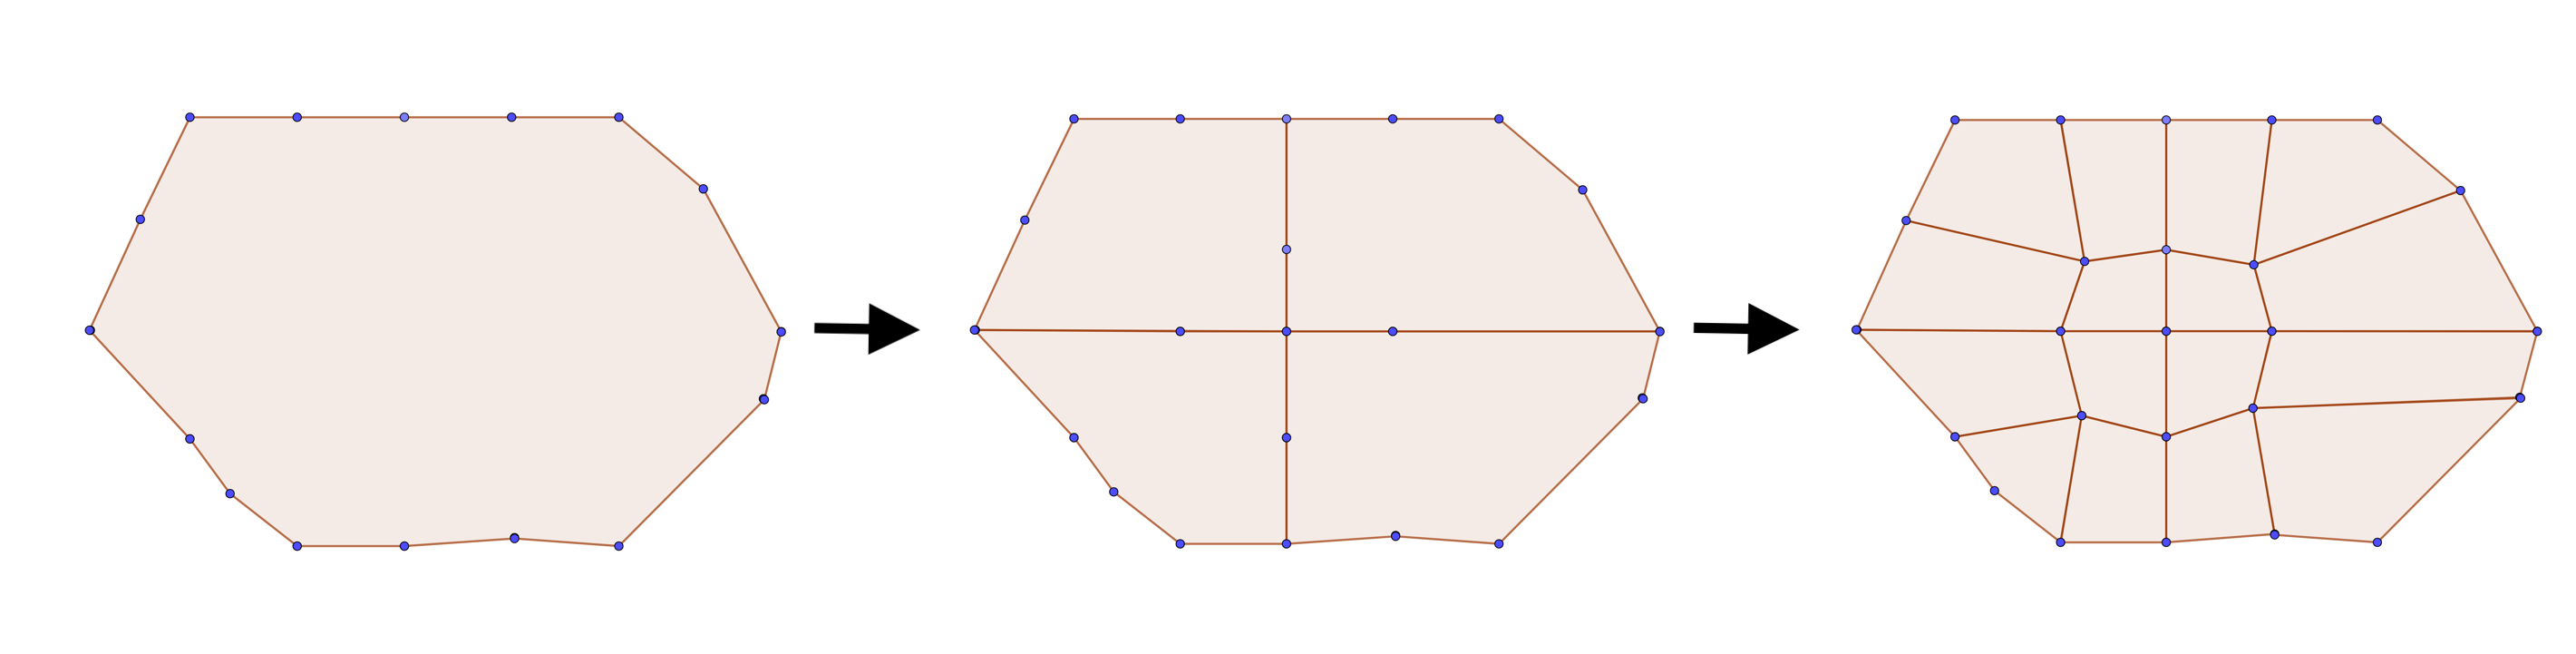
\includegraphics[width=0.75\textwidth]{RD_V/non_uniform_all_2.png}
% \captionsetup{labelformat=empty}
% \caption{Schematic illustration of the refinement process of a measurable space $\Omega$ into finer and finer partitions $\mathfrak{Q}_n$.
% Set $\Omega$ is uncountable, beige area. Partitions construt collections of finite subsets that are successively refined. Each collection is a finite
% measurable space. Two probability measures on $\Omega$ define two pmfs on each collection. Divergence of the two measures
% is obtained as limit of the divergences on the collections. }
% \end{figure}
% \end{frame}
%
%
% \begin{frame}{Computing divergence for random variables by quantization.}
% \loud{Divergence for random variables}
% \bit
% \item Let $X_1$ and $X_2$ be arbitrary random variables with values in $\mathbb{R}^d$, originating from probability
%  spaces with probability measutes $\mu^1$ and $\mu^2$.
% \item Divergence of $X_1$ and $X_2$ is divergence of their distributions:
% \begin{align*}
% D(X||Y):=D(\mu^1_{X}||\mu^2_{X}).
% \end{align*}
% \item For $N\in\mathbb{N}$, let $Q^N(X_1)$, $Q^N(X_2)$ denote their quantizes versions as in last lecture.
% \item By previous proposition:
% \begin{align}\label{DivRV}
% D(X_1||X_2)=\lim_{N\to\infty} D(Q^N(X_1)||Q^N(X_2)).
% \end{align}
% \item Could also take other sequences of quantizers $\tilde{Q}^N$ satifying assumptions of above proposition.
% \item[] \ALERT{$\iarrow$ Well defined digital-to-analog conversion for divergence of two random variables via
% any quantization scheme  that asymptotically generates the Borel-algebra}.
% \eit
%
%
%
% %
% %\loud{Sequence of partitions $\mathfrak{Q}_n$ for $\mathbb{R}^d$ }
% %\item For $N\in\mathbb{N}$ let $\Delta_N:=2^{-N}$.
% %According to \eqref{UniQuantCells}, for $i=(i_1,\dots,i_n)\in\mathbb{Z}^d$ let
% %\begin{align}\label{UniQuantCells}
% %\mathcal{C}_i^{N}:=\mathcal{C}_i(\Delta_N)= [i_1\cdot\Delta_N,(i_1+1)\cdot\Delta_N)\times\dots\times[i_d\cdot\Delta_N,(i_d+1)\cdot\Delta_N).
% %\end{align}n
% %\item For $N\in\mathbb{N}$ let
% %\[
% %I_N=\{i=(i_1,\dots,i_d)\in\mathbb{Z}^d\colon -N\cdot 2^N\leq i_k< N\cdot 2^N\:\forall k\}.
% %\]
% %\eit
% \end{frame}
%
%
% \begin{frame}{Mutual information}
% \loud{Recall: Mutual information in discrete case}
% \bit
% \item For discrete random-variables $X$ and $Y$ with alphabets $\mathcal{A}_X$ and $\mathcal{A}_Y$ , marginal pmfs $p_X$ and $p_Y$ and joint
% pmf $p_{(X,Y)}$, the mutual information $I(X,Y)$ satisifes
% \begin{align}\label{MutInfDisc}
% I(X,Y)=D(p_{X,Y}||p_X\times p_Y).
% \end{align}
% \item Here $p_X\times p_Y$ is the pmf on $\mathcal{A}_X\times\mathcal{A}_Y$ given as $p_X\times p_Y(x,y)=p_X(x)\cdot p_Y(y)$.
% \item Divergence $D$ now generally defined. \loud{Need to generalize $p_X\times p_Y$.}
% \eit
% \loud{$\iarrow$ Product measure}
% \bit
% \item Let $(\Omega_1,\Sigma_1)$ and $(\Omega_2,\Sigma_2)$ be measure spaces.
% \item \loud{Product $\sigma$-algebra} $\Sigma_1\otimes\Sigma_2$: Smallest $\sigma$-algebra that contains all sets $A\times B$, $A\in\Sigma_1$, $B\in\Sigma_2$.
% \item Let $\mu_1$ measure on $(\Omega_1,\Sigma_1)$ and $\mu_2$
% measure on $(\Omega_2,\Sigma_2)$, both $\sigma$-finite.
% %\item Assume that $\mu_1$ and $\mu_2$ are $\sigma$-finite, i.e. one can write $\Omega_1=\cup_i=1^\infty A_i$ with $A_i\in\Sigma_1$
% %and $\mu_1(\Sigma_1)<\infty$, same for $\mu_2$.
% %\item Example: Probability measures and Lebesgue measure are obviously $\sigma$-finite.
% \item \loud{Product measure:} There exists a unique measure $\mu_1\otimes \mu_2$ on $\Sigma_1\otimes\Sigma_2$ such that
% \begin{align*}
% \mu_1\otimes\mu_2(A\times B)=\mu_1(A)\cdot\mu_2(B),\quad \forall A\in \Sigma_1, \:\forall B\in\Sigma_2.
% \end{align*}
% \eit
% \end{frame}
%
% \begin{frame}{Product measures. Joint distribution. Marginal distribution. Independence.}
% \loud{Lebesgue measure on the Borel algebra as a product measure}
% \bit
% \item For the Borel-algebra, one has
% \begin{align}\label{BorelProduct}
% \mathfrak{B}(\mathbb{R}^{k+l})=\mathfrak{B}(\mathbb{R}^{k})\otimes\mathfrak{B}(\mathbb{R}^l); \quad
% \lambda_{k+l}=\lambda_{k}\otimes\lambda_l.
% \end{align}
% %for the Lebesgue measures \textit{as measures on the Borel algebras}.
% \item For larger $\sigma$-algebra of Lebesgue measurable set, needs to pass to completion.
% \eit
%
% \loud{Joint distribution, marginal distribution, independence:}
% \bit
% \item Let $X:\Omega\to\mathbb{R}^k$ and $Y:\Omega\to\mathbb{R}^l$ be random-variables on a probability spaces $(\Omega,\Sigma,\mu)$.
% \item It follows from \eqref{BorelProduct} that $(X,Y):\Omega\to\mathbb{R}^{k+l}$, $(X,Y)(\omega):=(X(\omega),Y(\omega))$ is a random variable.
% \item As in discrete case, distribution
% \[
% \mu_{X,Y}: \mathfrak{B}(\mathbb{R}^{k+l}) \to[0,1]
% \]
% of $(X,Y)$ is called \loud{joint distribution} of $X$ and $Y$, and
% $\mu_X$ and $\mu_Y$ are called \loud{marginal distributions}.
% \item $X$ and $Y$ are called \loud{independent} if
% \begin{align*}
% \mu_{X,Y}=\mu_X\otimes\mu_Y.
% \end{align*}
% \eit
% \end{frame}
%
% \begin{frame}{Mutual information in the general case}
% Divergence and product measure appearing in \eqref{MutInfDisc}
% are now generalized to the continuous case:
%
% \loud{$\iarrow$ Mutual information can be defined for two variables on a general proability space $(\Omega,\Sigma,\mu)$:}
% \bit
% \item For random variables $X$ and $Y$ on $\Omega$ put
% \begin{align}\label{MutInfCont}
% I(X;Y)=D(\mu_{X,Y}||\mu_X\otimes \mu_Y).
% \end{align}
% \item By \eqref{DivRV}, mutual information between random variables $X$, $Y$ is limit of mutual informations of their
% quantized versions $Q^N(X)$ and $Q^N(Y)$:
% \begin{align}\label{MutContLimit}
% I(X;Y)=\lim_{n\to\infty}I(Q^N(X); Q^N(Y)).
% \end{align}
% \item As for divergence: \ALERT{Any suitable family of quantizers on $\mathbb{R}^d$ gives a well established digital-to-analog conversion for mutual information.}
% \item Using \eqref{MutContLimit}, standard properties of mutual information like symmetry proved for discrete random variables
% carry over to the general case.
% \eit
% \end{frame}
%
%
%
% \begin{frame}{Mutual information via densities}
% \loud{Recall: } Formula for random variable having a \loud{density:}
% \begin{align}\label{EqDiffEntr}
% \lim_{N\to \infty}\left(H(Q^N(X))-dN\right)=h(X)
% \end{align}
% as a motivation for considering
% differences beteween entropies, i.g. mutual informations. Considerations are consistent:
% \begin{proposition}
% Let $(\Omega,\Sigma,\mu)$ be a probability space. Let $X, Y:\Omega\to \mathbb{R}^d$ be absolutely continuous random variables such that $(X,Y)$ is absolutely continuous. Let $f_X$ and
% $f_Y$ denote the densities of $X$ and $Y$ and let $f_{X,Y}$ denote the density of $(X,Y)$. Then one has
% \begin{align}\label{FormulaMIIntegral}
% I(X;Y)=\int_{\mathbb{R}}\int_{\mathbb{R}}f_{X,Y}(x,y)\log_2\left(\frac{f_{X,Y}(x,y)}{f_X(x)f_Y(y)}\right)dxdy.
% \end{align}
% \end{proposition}
% \vspace{-0.2cm}
% \loud{Proof}
% \vspace{-0.1cm}
% \bit
% \item General case: Use Radon-Nikodym theore, see book of Gray.
% \item Here:  Assume that \eqref{EqDiffEntr} can be applied.
% \eit
% \end{frame}
%
% \begin{frame}{Mutual information via densities. Proof.}
% \bit
% \item One has
% \begin{align*}
% I(X;Y)=&\lim_{N\to\infty}I(Q^{N}(X);Q^N(Y))\\
% =&\lim_{N\to\infty}\left(H(Q^{N}(X,Y))-H(Q^{N}(X))-H(Q^{N}(Y))\right)\\
% =&\lim_{N\to\infty}\left(H(Q^{N}(X,Y))-2dN)-(H(q^{N}(X))-dN)-(H(q^{N}(Y))-dN)\right).
% \end{align*}
% \item
% Thus by \eqref{EqDiffEntr}, one has
% \begin{align*}
% I(X;Y)
% =\int_{\mathbb{R}}\int_{\mathbb{R}}f_{X,Y}(x,y)\log_2(f_{X,Y}(x,y))dxdy-
% \int_{\mathbb{R}}f(x)\log_2(f(x))dx-\int_{\mathbb{R}}f(y)\log_2(f(y))dy.
% \end{align*}
% \item For the marignal denities $f_X$ and $f_Y$, one has
% \begin{align*}
% f_X(x)=\int_{\mathbb{R}}f_{X,Y}(x,y)dy;\quad f_X(y)=\int_{\mathbb{R}}f_{X,Y}(x,y)dx,\quad\text{allmost everywhere.}\qed
% \end{align*}
% \eit
% Similarly: \loud{Definition of divergences are consistent} if $X$ and $Y$ have densities.
% \end{frame}
%
%
% \begin{frame}{Informational rate-distortion function, general case}
% Mutual information defined $\iarrow$ Can define informational rate distortion function as before.
% \begin{definition}
% Let $(\Omega,\Sigma,\mu)$ be a probability space and let $X:\Omega\to\mathbb{R}$ be a continuous
% random variable (r.v.). Let $d$ be a distortion function. The informational rate distortion function is defined as
% \begin{align*}
% R^{(I)}(D):=\inf\bigl\{&I(X;\hat{X})\colon  \text{$\hat{X}$ is an $\mathbb{R}$-valued r. v.  and there exists an $\mathbb{R}^2$-valued r. v. $Z=(Z_1,Z_2)$}\\ &\text{on some probability space with probability measure $\nu$ such that $Z_1\stackrel{d}{=} X$ and $Z_2\stackrel{d}{=} \hat{X}$} \\ &\text{and such that
% $\int_{\mathbb{R}^2}d(x,\hat{x})d\nu_Z(x,\hat{x})<D$. }
% \bigr\}
% \end{align*}
% \end{definition}
% \vspace{-0.2cm}
% \bit
% \item Recall: $X\stackrel{d}{=} Y$ for r.v. $X$ and $Y$ means that $X$ and $Y$ have the same distribution.
% \item Definition is consistent with previous definition of $R^{(I)}(D)$ for the discrete case.
% \item As in discrete case, can also define $R^{(I)}(D)$ using conditional distribution instead of $Z$.
% \item However: (Regular versions of) conditional expectation not introduced in this lecture.
% %\item See standard textbooks on probability theory.
% %\item Suffices to work with joint distribution $Z$.
% \eit
% \end{frame}
%--------------------end took out by JR

\subsection{Source codes and rate-distortion functions for general random variables.}
\begin{frame}
 \vspace{12.0ex}
\begin{center}
\begin{beamercolorbox}[sep=12pt,center]{part title}
\usebeamerfont{section title}\insertsubsection\par
\end{beamercolorbox}
\end{center}
\end{frame}

\begin{frame}{Lossy source codes for general sources $X$} 
Let $X$ be a random-variable with values in $\mathbb{R}^d$ and distribution $\mu_X$. 
%\vspace{-0.2cm}
\loud{Lossy source code $Q=(\alpha,\gamma,\beta)$ for $X$}
\bit
\item Same definition as before. But: Quantization defined as mapping on the whole $\mathbb{R}^d$.
\item $\alpha: \mathbb{R}^d\to \mathcal{I}_K:=\{1,\dots,K\}$, \loud{quantization}
\item $\gamma$: \loud{Lossless mapping}. Uniquely decodable code for $\mathcal{I}_K$. 
\item $\beta: \mathcal{I}_K\to\mathbb{R}^d$, \loud{inverse quantization}. 
\eit

\loud{Main difference to case of finite alphabets:} 
\bit
\item One never has: $\beta(\alpha(x))\neq x$.
\item[\iarrow] If one assumes that $X$ does not attain only finitely many values $\mathcal{A}_X$,  there is always loss in information.
\item Lossless source codes do not exist for general random variables.
\eit
\vspace{-0.2cm}
\loud{Rate of a source code:}
\bit
\item Defined as before: $\mu_X$ and $\alpha$ induce discrete probability distribution on $\mathcal{I}_K$. 
\item [\iarrow] Rate is average expected codeword-length of $\gamma$. 
\eit


\end{frame}

\begin{frame}\frametitle{Lossy source codes: Distortion}
\bit
\item Fix a distortion measure $d$ on $\mathbb{R}$, get additive extension $d_N$ on $\mathbb{R}^N$. 
\item The distortion $\delta(Q)$ of a source code $Q$ is defined as the expected mean squared Euclidean distance between original and 
reconstructed symbols  
\begin{align*}
\delta(Q)=\int_{\mathbb{R}^N}d_N(s,\beta(\alpha(s)))d\mu_X(s).
\end{align*}
\item Define a discrete random variable $Y$ on $\Omega$ by $Y(\omega):=\beta(\alpha(X(\omega)))$, quantization of $X$.
\item Let $Z:=(X,Y)$. $Z$ is a random variable; never absolutely continuous. 
\item Distribution $\mu_{Z}$ of $Z$ is a probability measure on $\mathbb{R}^{N}\times\mathbb{R}^N$.
%If $X$ is continous, $Z$ is a mixture of 
%a continuous and discrete random variable, does not have a density.
\item By definition, one has
\begin{align*}
\delta(Q)=\int_{\mathbb{R}^N\times\mathbb{R}^N}d_N(x,\hat{x})d\mu_Z(x,\hat{x}).
\end{align*}
\item For $N=1$, last equation is consistent with distortion term in informational rate distortion function. 
\eit 
\end{frame}


\begin{frame}\frametitle{Lossy source codes: Quantization cells}
Let $Q=(\alpha,\gamma,\beta)$ be a source code. 
\begin{itemize}
\item For $i\in\mathcal{I}_K$, the set 
$C_i:=\alpha^{-1}(i) $
is called the \loud{quantization cell} of index $i$.
\item The value 
$\hat{x}_i:=\beta(i)$ is called the reconstructed value of index $i$. 
\item The quantization cells $C_i$ are pairwise disjoint and their union is $\mathbb{R}^N$. 
\item One has 
\begin{align}\label{RDQuantCells}
\delta(Q)=\sum_{i\in\mathcal{I}_K}\int_{C_i}\left\|x-\hat{x}_i\right\|^2d\mu_X(x),\quad r(Q)=\sum_{i\in\mathcal{I}_K}|\gamma(i)|\mu_X(C_i).
\end{align}
\begin{figure}
\centering
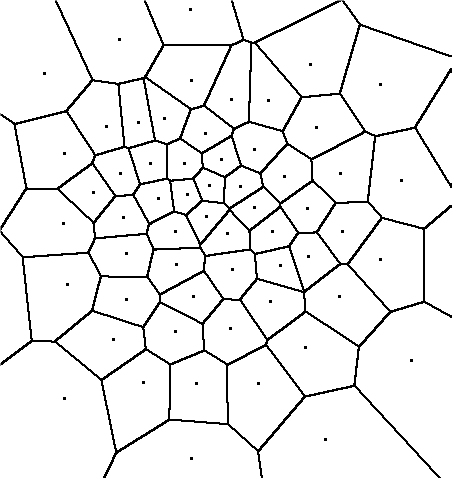
\includegraphics[width=0.12\textwidth]{RD_V/quant_cells.png}
\captionsetup{labelformat=empty}
\caption{Example for quantization cells and reconstruction points in $\mathbb{R}^2$.}
\end{figure}
\end{itemize}
\end{frame}




\begin{frame}{Rate distortion function and fundamental source coding theorem. General case.}  
\loud{Rate distortion function}
\bit
\item Let $X$ be an $\mathbb{R}^N$-valued random variable and let $Q$ be a source code for $X$.
\item For $D\in [0,\infty)$, one puts
\begin{align*}
R(D)= \inf\{r(Q)\colon \text{$Q$ is a source code with $\delta_N(Q)\leq D$}\}.
\end{align*}
\item If support of $\mu_X$, i.e. $\{x\in\mathbb{R}^N\colon \mu_X(x)\neq 0$\} is uncountalbe, $R(D)$ goes to infinity as $D\to 0$.
\item In particular: $R(D)$ goes to infinity as $D\to 0$ if $X$ is an absolutely continuous random variable.
\eit

\loud{Setup for fundamental lossless source coding theorem:} Analog to discrete case. 
\bit
\item Let $X$ be an $\mathbb{R}$-valued random variable. 
\item Consider joint coding of $N$ independent realizations of $X$, i.e. 
joint coding of $\mathbb{R}^N$-valued sources $X^N=(X_1,\dots,X_N)$ with 
process $iid$, $X_i\stackrel{d}{=}X$ for all $i$.
\item If $Q$ is a source code for $X^N$, rate $r(Q)$ is meant as rate per symbol, i. e. normalized with $1/N$.
\item Fix a distortion function $d$ on $\mathbb{R}$, extend $d$ to additive distortion function on $\mathbb{R}^N$.  
\eit 
\end{frame}

\begin{frame}{Fundamental source coding theorem for general random variables.}
\begin{theorem} 
\begin{enumerate}
\item The informational rate distortion function $R^{(I)}$ is always a \loud{lower bound} for the rate distortion function: 
For every $N\in\mathbb{N}$ and every source code $Q_N$ for $X^N$ one has
\begin{align}\label{BoundRate}
r(Q_N)\geq R^{(I)}(\delta(Q_N)). 
\end{align}
\item The bound \eqref{BoundRate} is \loud{asymptotically achievable}: For every $D>0$, every $\epsilon>0$ and every $R'>R^{(I)}(D)$, one can achieve 
\begin{align*}
\delta(Q_N)\leq D+\epsilon, \quad r(Q_N)\leq R'
\end{align*}
for some sequence $Q_N$  of source codes for $X^N$ where $N$ can be chosen arbitrarily large.    
\end{enumerate} 
\end{theorem}
\loud{Proof: Proceed exactly as in discrete case.}
\bit
\item Mutual information has same properties as in discrete case.% by \eqref{MutContLimit}.
\item Law of large number holds for $X^N$ $\iarrow$ Ensemble set and random-coding can be constructed as in the discrete setting. 
\eit 
\end{frame}


\subsection{Rate distortion function for a scalar Gaussian source}

\begin{frame}
 \vspace{12.0ex}
\begin{center}
\begin{beamercolorbox}[sep=12pt,center]{part title}
\usebeamerfont{section title}\insertsubsection\par
\end{beamercolorbox}
\end{center}
\end{frame}



\subsubsection{Basic properties of the Gaussian Distribution}

\begin{frame}{Review: Definition of the scalar Gaussian distribution}
\loud{The Gaussian function} 
\bit
\item For $\sigma\in(0,\infty)$, the \loud{Gaussian function} is defined as 
\begin{align*}
\phi_{\sigma}(x):=\frac{1}{\sqrt{2\pi\sigma^2}}\exp\left(-\frac{x^2}{2\sigma^2}\right).
\end{align*}
%\item For any $\mu\in\mathbb{R}$, one has 
%\begin{align*}
%\int_{\mathbb{R}}\phi_\sigma(x-\mu)dx=1;\quad \int_{\mathbb{R}}\phi_\sigma(x-\mu)xdx=\mu;\quad \int_{\mathbb{R}}\phi_\sigma(x-\mu)(x-\mu)^2dx=\sigma^2.
%\end{align*}
\item Integration of $\phi_{\sigma}(x-\mu)$ defines a probability measure on $\mathfrak{B}(\mathbb{R})$ with mean $\mu$ and variance $\sigma^2$. 
\eit

\loud{Gaussian distributed random variables}
\bit
\item An $\mathbb{R}$-valued random variable $X$ is \loud{Gaussian distributed with mean $\mu$ and variance $\sigma$}, 
\begin{align*}
X\sim \mathcal{N}(\mu,\sigma^2), 
\end{align*}
if 
$X$ is absolutely continuous and its density $f_X$ satisfies $f_X(x)=\phi_{\sigma}(x-\mu)$ almost everywhere.
\item Gaussian distribution arguably \loud{most important model distribution}. 
\item One important  reason: \loud{Central limit theorem}. 
\eit
\end{frame}









\begin{frame}
\begin{proposition}[Differential entropy for the Gaussian source.]
\begin{enumerate}
\item The differential entropy of a normally distributed random variable $X\sim N(\mu,\sigma^2)$ satisfies
\begin{align}\label{EqDiffEntrGV}
h(X)= \frac{1}{2}\log_2(2\pi\sigma^2 e).
\end{align}
\item All absolutely continuous sources $Y$ having a finite differential entropy and having finite variance $\sigma^2$ satisfiy
\begin{align}\label{IneqEntr}
h(Y)\leq \frac{1}{2}\log_2(2\pi\sigma^2 e).
\end{align}
The Gaussian distribution $\mathcal{N}(\mu,\sigma^2)$ maximes the differential entropy for a given variance. 
\end{enumerate}
\end{proposition}
\bit
\item Using \loud{Shannon lower bound}: Will be shown that Gaussian iid process is `most difficult to code for high rates' among 
all iid processes with same variance.
\item [\iarrow] Heuristically consistent with maximalization \eqref{IneqEntr} and meaning of entropy from discrete case.  
\eit

\end{frame}

\begin{frame}{Computation of differential entropy of scalar Gaussian source.}
\bit
\item For $X\stackrel{d}{=} N(\mu,\sigma^2)$ one computes
\begin{align*}
h(X)=&-\int_{\mathbb{R}}\phi_{\sigma}(x-\mu)\log_2(\phi_{\sigma}(x-\mu))dx\\
=&-\int_{\mathbb{R}}\phi_{\sigma}(x)\log_2(\phi_{\sigma}(x))dx\\
=& \frac{1}{\ln(2)}\cdot\frac{1}{\sqrt{2\pi\sigma^2}}\int_{\mathbb{R}}\exp\left(-\frac{x^2}{2\sigma^2}\right)\left(\ln(\sqrt{2\pi\sigma^2})+\frac{x^2}{2\sigma^2}\right)dx\\
=&\frac{1}{\ln(2)}\cdot\left(\ln(\sqrt{2\pi\sigma^2})\int_{\mathbb{R}}\phi_\sigma(x)dx+\frac{1}{2\sigma^2}\int_{\mathbb{R}}\phi_\sigma(x)x^2dx\right)\\
=&\frac{1}{\ln(2)}\cdot\left(\ln(\sqrt{2\pi\sigma^2})+\frac{1}{2}\right)\\
=&\frac{1}{2\ln(2)}\cdot\left(\ln(2\pi\sigma^2)+1\right)\\ 
=&\frac{1}{2}\log_2(2\pi\sigma^2 e).
\end{align*}
\eit
\end{frame} 

\begin{frame}{Scalar Gausian distribution maximes differential entropy}
\loud{Proof}
\bit
\item Let $Y$ be any absolutely continous distribution of variance $\sigma^2$ and probability density function $g$.
\item One has 
\begin{align*}
0\leq D(g||\phi_\sigma)=&\int_{\mathbb{R}}g(x)\log_2\left(g(x)/\phi_\sigma(x)\right)dx\\
=&\int_{\mathbb{R}}g(x)\log_2(g(x))dx-\int_{\mathbb{R}}g(x)\log_2(\phi_\sigma(x))dx\\
=&-h(g)+\frac{1}{\ln(2)}\int_{\mathbb{R}}g(x)\left(\ln(\sqrt{2\pi\sigma^2})+\frac{x^2}{2\sigma^2}\right)dx\\
=&-h(g)+\frac{1}{\ln(2)}(\ln(\sqrt{2\pi\sigma^2})\int_{\mathbb{R}}g(x)dx+\frac{1}{2\sigma^2}\int_{\mathbb{R}}x^2g(x)dx)\\
=&-h(g)+\frac{1}{\ln(2)}(\ln(\sqrt{2\pi\sigma^2})+1/2)\\
=&-h(g)+h(\mathcal{N}(0,\sigma^2)).
\end{align*}
\eit
\end{frame}

\subsubsection{Rate distortion function for scalar Gaussian sources}
\begin{frame}{Rate-distortion function of a Gaussian source}
\begin{theorem}
Let $X$ be an $\mathbb{R}$-valued Gaussian source of mean $\mu$ and variance $\sigma^2$, i.e. $X\stackrel{d}{=} \mathcal{N}(\mu,\sigma^2)$. Then one has 
\begin{align}\label{RDGauss}
R(D)=\begin{cases} &0, \text{if $D\geq \sigma^2$} \\ &\frac{1}{2}\log_2\left(\frac{\sigma^2}{D}\right), \text{else.} \end{cases}
\end{align}
\end{theorem}
\bit
\item [\iarrow] \loud{Explicit formula for the rate-distortion function of a very important source, probably most 
important model source!}
\eit
\vspace{-0.2cm}
\loud{Many application of \eqref{RDGauss} and its extensions will be given:} 
\bit
\item Can explicitly quantify vector quantization advantage for Gaussian sources.
\item Can explicity compare optimal transform coding 
scheme with general vector quantization for Gaussian sources. 
\item Transform coding: Cornerstone of modern image- and video-codecs.
 \eit
\end{frame}

\begin{frame}{Rate-distortion function of a scalar Gaussian source}
\loud{Lower bound for $R^{(I)}(D)$: }
\bit
\item Let $\hat{X}$ be a random-variable that joint distribution of $X$ and $\hat{X}$ satisfies the distortion constraint. Then: 
\begin{align}
I(X;\hat{X})=h(X)-h(X|\hat{X})
= & h(X)-h(X-\hat{X}|\hat{X})\nonumber\\
\geq & h(X)- h(X-\hat{X})\nonumber\\
\geq & h(X) - \sup_{\{Y\colon var(Y)<D\}}h(Y)\nonumber\\
\geq & h(X) - \frac{1}{2}\log_2(2\pi\sigma^2 e)\label{GaussRDI}\\
=& \frac{1}{2}\log_2\left(\frac{\sigma^2}{D}\right)\label{GaussRDII}. 
\end{align}
\item Here, \eqref{GaussRDI} follows from \eqref{IneqEntr} and \eqref{GaussRDII} follows from \eqref{EqDiffEntrGV}. 
\item Justsification of other (in)equalities. See below. 
\eit

\end{frame}




\begin{frame}{Rate-distortion function of a 1-D Gaussian source.}
\loud{Proof of achievability.}
\bit
\item Let $\hat{X}$ be a Gaussian source such that
\bit
\item $\hat{X}\stackrel{d}{=} \mathcal{N}(0,\sigma^2-D)$.
\item $X-\hat{X}\stackrel{d}{=} \mathcal{N}(0,D)$.
\item $\hat{X}$ and $X-\hat{X}$ are independent.
\eit
\item \textbf{Exercise: } Show that $\hat{X}$ exists. Use that convolution of Gaussians is Gaussian, mean and variance add up. 
\item One has
\begin{align*}
I(X;\hat{X})=&h(X)-h(X|\hat{X})\\
=&h(X)-h(X-\hat{X}|\hat{X})\\
=&h(X)-h(X-\hat{X})\\
=& \frac{1}{2}\log_2\left(\frac{\sigma^2}{D}\right).
\end{align*}
\eit
\end{frame}

\begin{frame}{Rate distortion function of scalar Gaussian source. Remarks on proof.}
\loud{Remark on the proof: }
\bit
\item  Previous (in)equalities are easily verified for \loud{discrete case}.
\item Using \eqref{MutContLimit},  they extend easily to present case. 
\item One does not even need to define conditional entropy for continuous case.
\item  Argue exactly as in the proof of \eqref{FormulaMIIntegral}, using that \eqref{EqDiffEntr} also holds for the Gaussian distribution. 
\eit
\end{frame}

\begin{frame}{Rate-distortion function of a Gaussian source: Vector quantization advantage}
Let $X$ be a 1-D Gaussian source.
\bit
\item \loud{Scalar quantization:} Rate-distortion function of $X$ or of $X^N$ when coding each component of $X^N$ separately (i.e. concatenation of 1-D source-codes).  
\item Let $R_{sq}(D)$ be rate-distortion function for scalar quantization of $X$. 
\item After Christmas, \loud{High rate approximation of Gish and Pierce: }:
One has
\[
R_{sq}(D)\approx \frac{1}{2}\log_2\left(\frac{\pi e}{6}\cdot\frac{\sigma^2}{D}\right), \quad\text { as $R\to\infty$.}
\]
\item[\iarrow] Compare to rate-distortion function of $X$:  
\begin{align}\label{VQ_Advantage}
R_{sq}(D)-R(D)\approx \frac{1}{2}\log_2\left(\frac{\pi e}{6}\right)\approx 1/4,  \quad\text { as $R\to\infty$.}
\end{align}
\eit
\alert{\iarrow \textbf{Vector quantization advantage of 1/4 bit per sample for Gaussian source at high rates.}}
\bit
\item Equation \eqref{VQ_Advantage} holds for more general sources by \textit{asymptotic tightness of Shannon lower bound}. 
\eit
\end{frame}

\end{document}
